\clearpage
\maketitlesupplementary
\appendix

\setcounter{section}{0}
\setcounter{equation}{0}
\setcounter{figure}{0}
\setcounter{table}{0}
\renewcommand{\thefigure}{S.\arabic{figure}}
\renewcommand{\thetable}{S.\arabic{table}}
\renewcommand{\theequation}{S.\arabic{equation}}


\section{Acknowledgments}

We thank Michael Zollhöfer for his initial involvement in project discussions.
We also thank Jeff Tan, Jianyuan Wang, Jay Karhade, Jinghao (Jensen) Zhou, Yifei Liu, Shubham Tulsiani, Khiem Vuong, Yuheng Qiu, Shibo Zhao, Omar Alama, Andrea Simonelli, Corinne Stucker, Denis Rozumny, Bardienus Duisterhof, and Wenshan Wang for their insightful discussions, feedback, and assistance with parts of the project.
Lastly, we appreciate the support for compute infrastructure from Julio Gallegos, Tahaa Karim, and Ali Ganjei.

\vspace{0.4em}

\noindent\textbf{\textcolor{citegray}{Funding at Carnegie Mellon University:}} Nikhil's time and parts of this work at CMU was supported by Defense Science and Technology Agency (DSTA) Contract {\scriptsize\texttt{\#DST000EC124000205}}, DEVCOM Army Research Laboratory (ARL) SARA Degraded SLAM {\scriptsize\texttt{CRA W911NF-20-S-0005}}, and the Intelligence Advanced Research Projects Activity (IARPA) via Department of Interior/Interior Business Center (DOI/IBC) contract number {\scriptsize\texttt{140D0423C0074}}. The U.S. Government is authorized to reproduce and distribute reprints for Governmental purposes notwithstanding any copyright annotation thereon. Disclaimer: The views and conclusions contained herein are those of the authors and should not be interpreted as necessarily representing the official policies or endorsements, either expressed or implied, of IARPA, DOI/IBC, or the U.S. Government. 
The compute required for this work at CMU was supported by a hardware grant from Nvidia and used PSC Bridges-2 through allocation {\scriptsize\texttt{cis220039p}} from the Advanced Cyberinfrastructure Coordination Ecosystem: Services \& Support (ACCESS) program.






\vspace{-0.8em}

\section{Implementation Details}

We use the AdamW \cite{KingmB2015} optimizer with a peak learning rate of $5\cdot10^{-6}$ for the pre-trained DINOv2 encoder \cite{OquabDMVSKFHMEABGHHLMRSSXJMLJB2024}, and $10^{-4}$ for everything else.
For the learning rate schedule, we employ a 10\% linear warmup to the peak and subsequently use a half-cycle cosine decay to a $100\times$ lower value.
For the optimizer, we also use a weight decay of 0.05, $\beta_1 \!=\! 0.9$, and $\beta_2 \!=\! 0.95$.
For every batch, the input images and dense geometric quantities are resized and cropped so that the maximum dimension is 518 pixels and aspect ratio is randomized from 3:1 to 1:2.
We use color jitter, Gaussian blur, and grayscale conversion as augmentations.
We further employ mixed precision training and gradient checkpointing for DINOv2 encoder to improve training efficiency and GPU memory utilization.
We also use gradient norm clipping with a threshold of 1 for additional training stability.
Lastly, we use a dynamic batching scheme where the batch size is changed based on the number of views in a batch.
We find that it is effective to train the model with a two-stage curriculum (420K steps):
(1) 6 days on 64 H200-140GB GPUs with an effective batch size varying from 768 to 1536 with the number of views varying from 4 to 2, respectively, and
(2) 4 days on 64 H200-140GB GPUs with a 10$\times$ lower peak LR and an effective batch size that varies from 128 to 1536 with views varying from 24 to 2, respectively.
The training setup for the ablations presented in \cref{para:insights} is the same as above where the only difference is the effective batch size (8$\times$ lower but leading to sufficient convergence).

\vspace{-0.7em}

\section{Additional Evaluation}

\paragraph{Speed \& Memory Profiling:} We present profiling results for \coolname and other concurrent models in \cref{fig:profiling}.

\vspace{-0.15em}

\paragraph{Flexibility of Input Configurations:}

We present a representative set of input configurations for \coolname in \cref{tab:supplementary_mapanything_input_variants}, where the performance of \coolname improves as more modalities are provided.
The universal training of \coolname with varying selection probabilities for geometric inputs as 6 factors (as described in \cref{para:aug_training}) enables support for 64 exhaustive input combinations.
While we primarily benchmark cases where the input modality is available for all views, \coolname can also support optional geometric inputs for a subset of the input views.

\vspace{-0.15em}




\paragraph{Comparison of \coolname Variants:}

We provide a comparison between different variants of \coolname in \cref{fig:mapa_variants_comparison_graphs}, where the performance of VGGT~\cite{WangCKVRN2025} is provided as a baseline.
First, we show that our two-stage training with covisibility-based view sampling is very effective, where the \coolname model trained for up to 4 views as input already shows strong generalization to a significantly higher number of views.
We also compare the performance of our different open-source models, where, as described in \cref{tab:datasets}, the Apache model is trained on 6 datasets, while the CC-BY-NC one is trained on 13.
While we observe a decrease in performance, the Apache variant is still competitive with the VGGT baseline and its performance further improves as additional geometric inputs are provided.
We also provide a comparison between the various versions of the publicly released models in \cref{fig:v1_1_vs_v1}.

\vspace{-0.15em}

\paragraph{Design Choices:}

As shown in \cref{tab:ablations_loss_attention}, log scaling and alternating attention are key for strong performance when evaluating with 50 views, well beyond the 4 used in training.

\vspace{-0.15em}

\paragraph{Qualitative Examples:}

\cref{fig:qual_diversity} and \cref{fig:qual_geometric_inputs} showcase the versatility of \coolname.

\vspace{-0.15em}

\paragraph{Comparison with Concurrent Models:}

\cref{fig:v1_1_bench_average} showcases the average results, while \cref{fig:v1_1_bench_img_only_per_dataset} and \cref{fig:v1_1_bench_multi_modal_per_dataset} show the performance for each individual dataset.





\begin{figure*}[t]
    \centering
    \begin{subfigure}{0.49\textwidth}
        \centering
        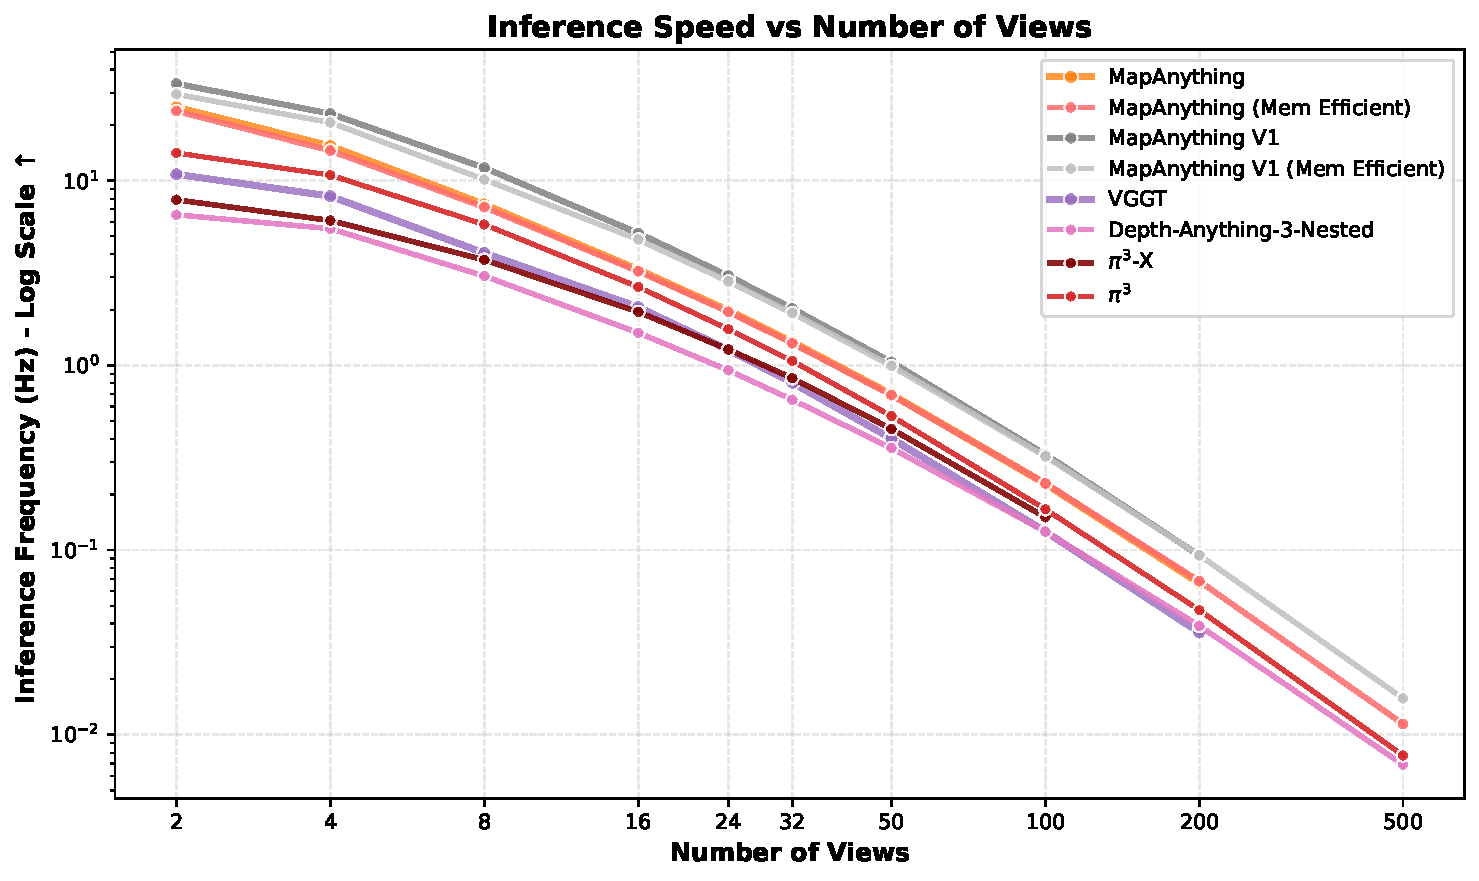
\includegraphics[width=\linewidth]{figs/Profiling_Results/profiling_speed.pdf}
    \end{subfigure}
    \hfill %
    \begin{subfigure}{0.49\textwidth}
        \centering
        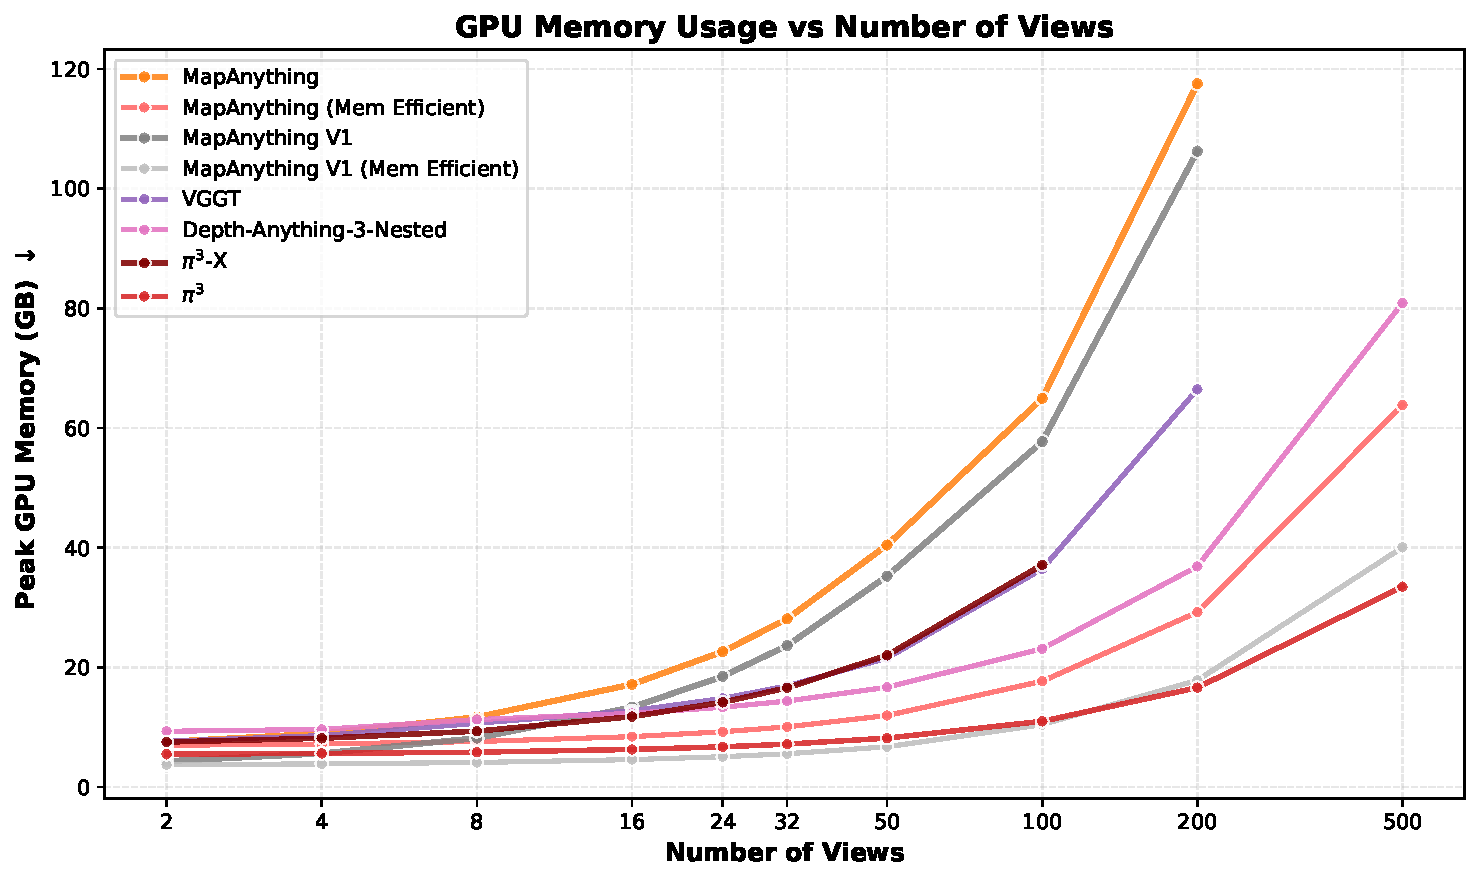
\includegraphics[width=\linewidth]{figs/Profiling_Results/profiling_memory.pdf}
    \end{subfigure}

    \caption{\label{fig:profiling}
    \textbf{\coolname shows the best speed and memory usage profile in comparison to latest concurrent state-of-the-art multi-view feed-forward reconstruction models.} 
    We profile all the models on a H200-140GB GPU using appropriate floating point precision autocast.
    Upon profiling the naive inference call of \coolname and comparing to concurrent methods, we notice a memory bottleneck in the dense per-pixel regression across views, since our implementation of the dense head is closer to the original DPT~\cite{RanftBK2021}.
    To alleviate this issue, i.e., in \coolname (Mem Efficient), we run the per-view decodings in a mini-batched loop, where in the above profiling the mini-batch size is 1.
    We find that this looping leads to negligible trade-off in speed while significantly reducing the memory usage.
    }
\end{figure*}

\begin{figure*}[!t]
    \centering
    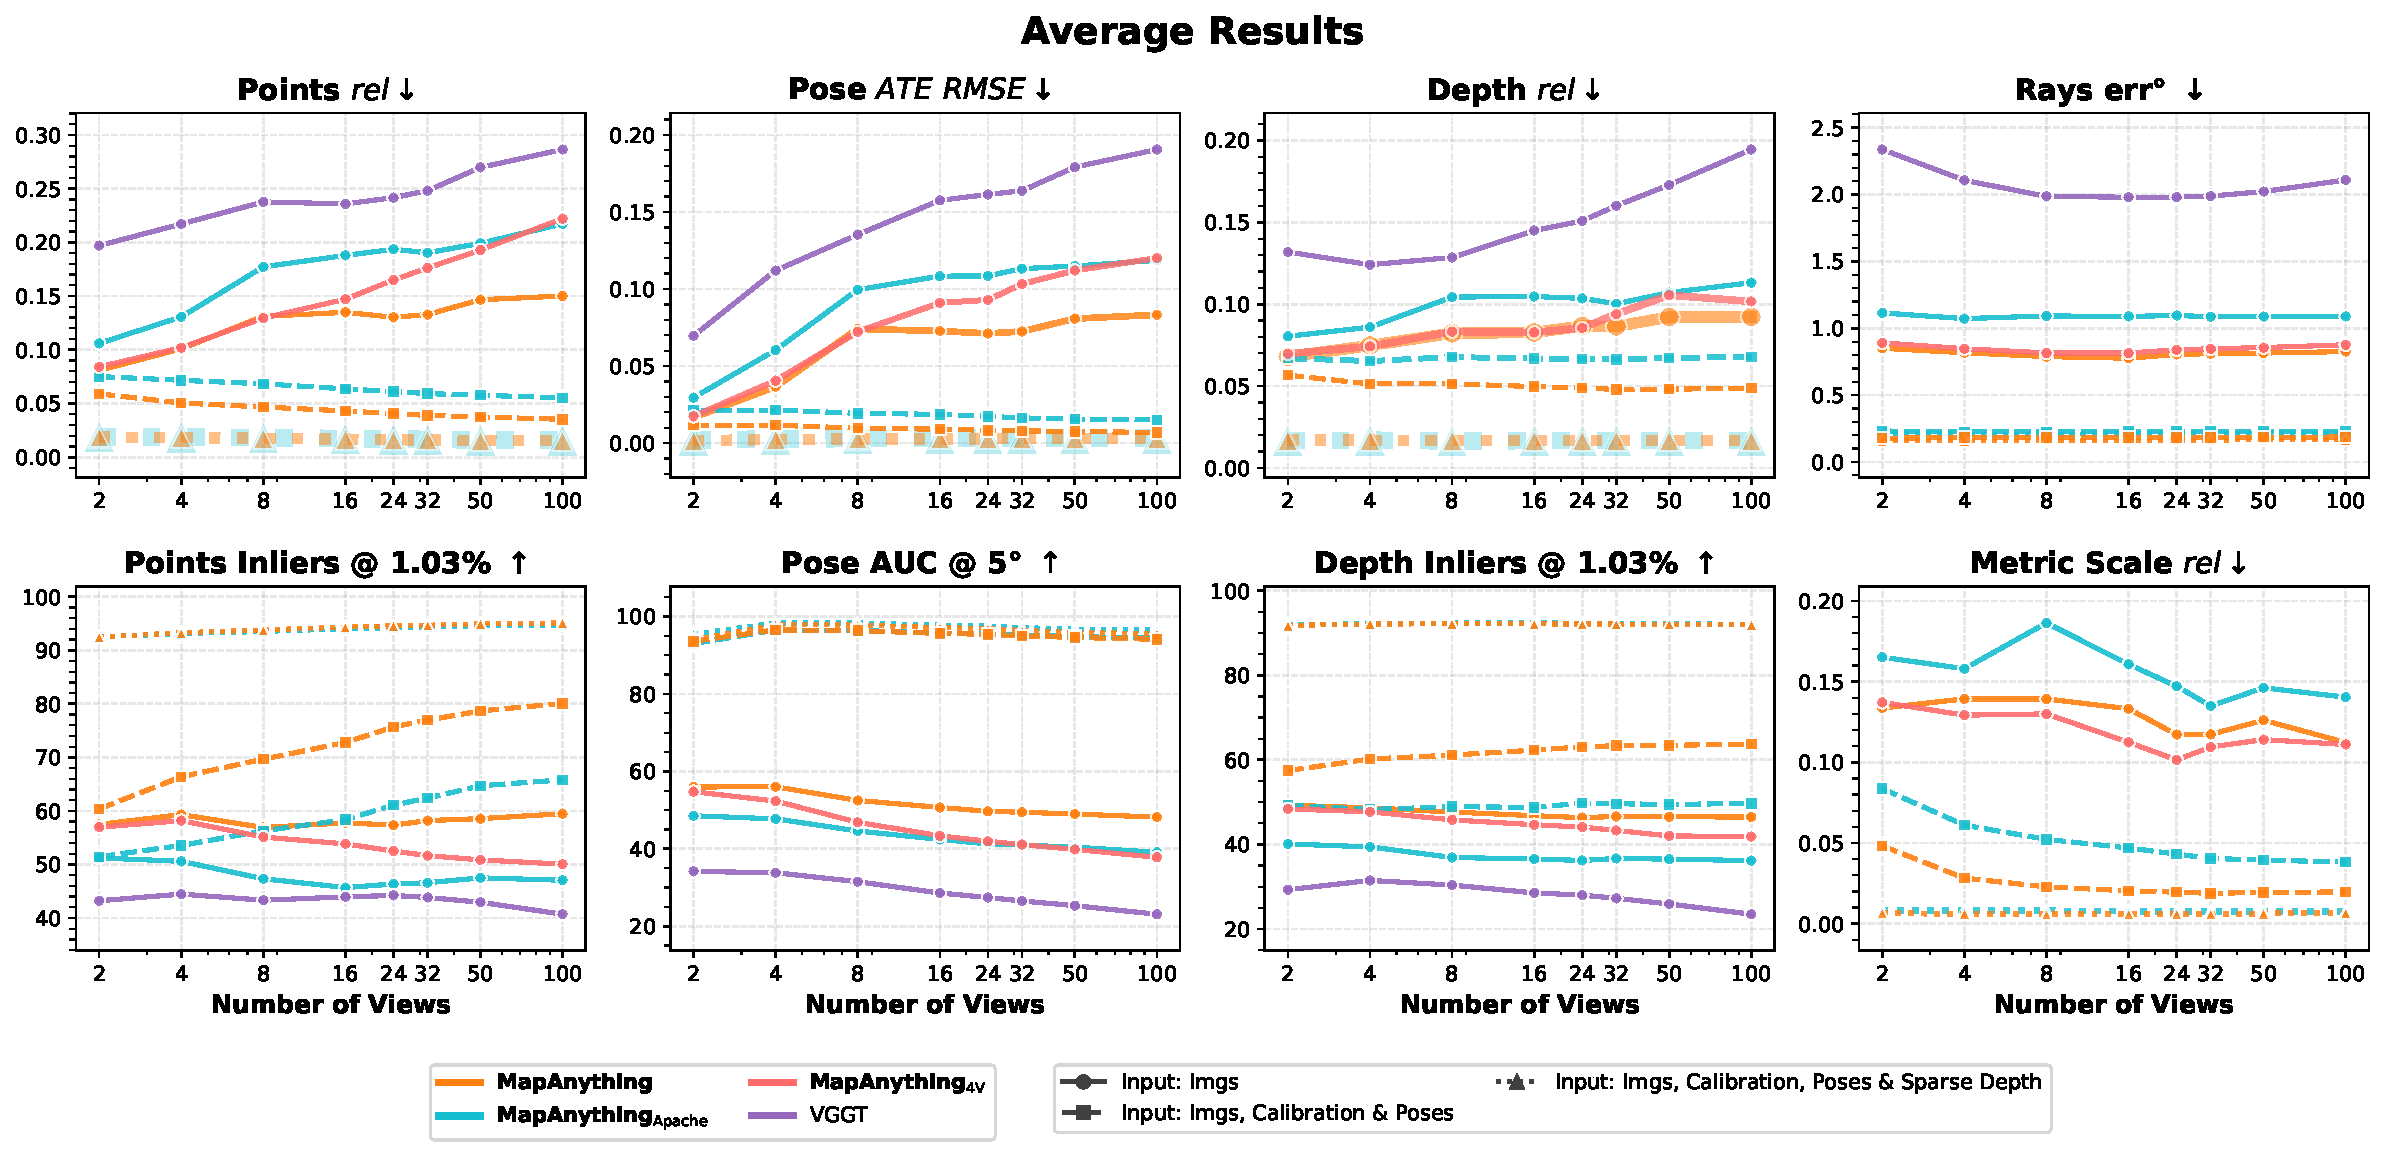
\includegraphics[trim={0cm 0cm 0cm 0.9cm},clip,width=\linewidth]{figs/V1_1_Benchmarking/v1_1_bench_apache/results_v1_1_bench_apache_average.pdf}
    \caption{\label{fig:mapa_variants_comparison_graphs}%
    \textbf{The Apache and first stage (up to 4 views) training variants of \coolname show strong dense multi-view reconstruction for input views ranging from 2 to 100 and under different input configurations.}
    We report the absolute relative error ($\absrel$), the inlier ratio at a relative threshold of $1.03\%$ ($\threshI$), the average aligned trajectory error ($ATE~RMSE$), the area under the curve at an error threshold of 5° ($AUC@5$), and the average angular error ($err$) in degrees (°), averaged over ETH3D, ScanNet++ v2 \& TAv2.
    }
\end{figure*}

\clearpage

\begin{figure*}[!t]
    \centering

    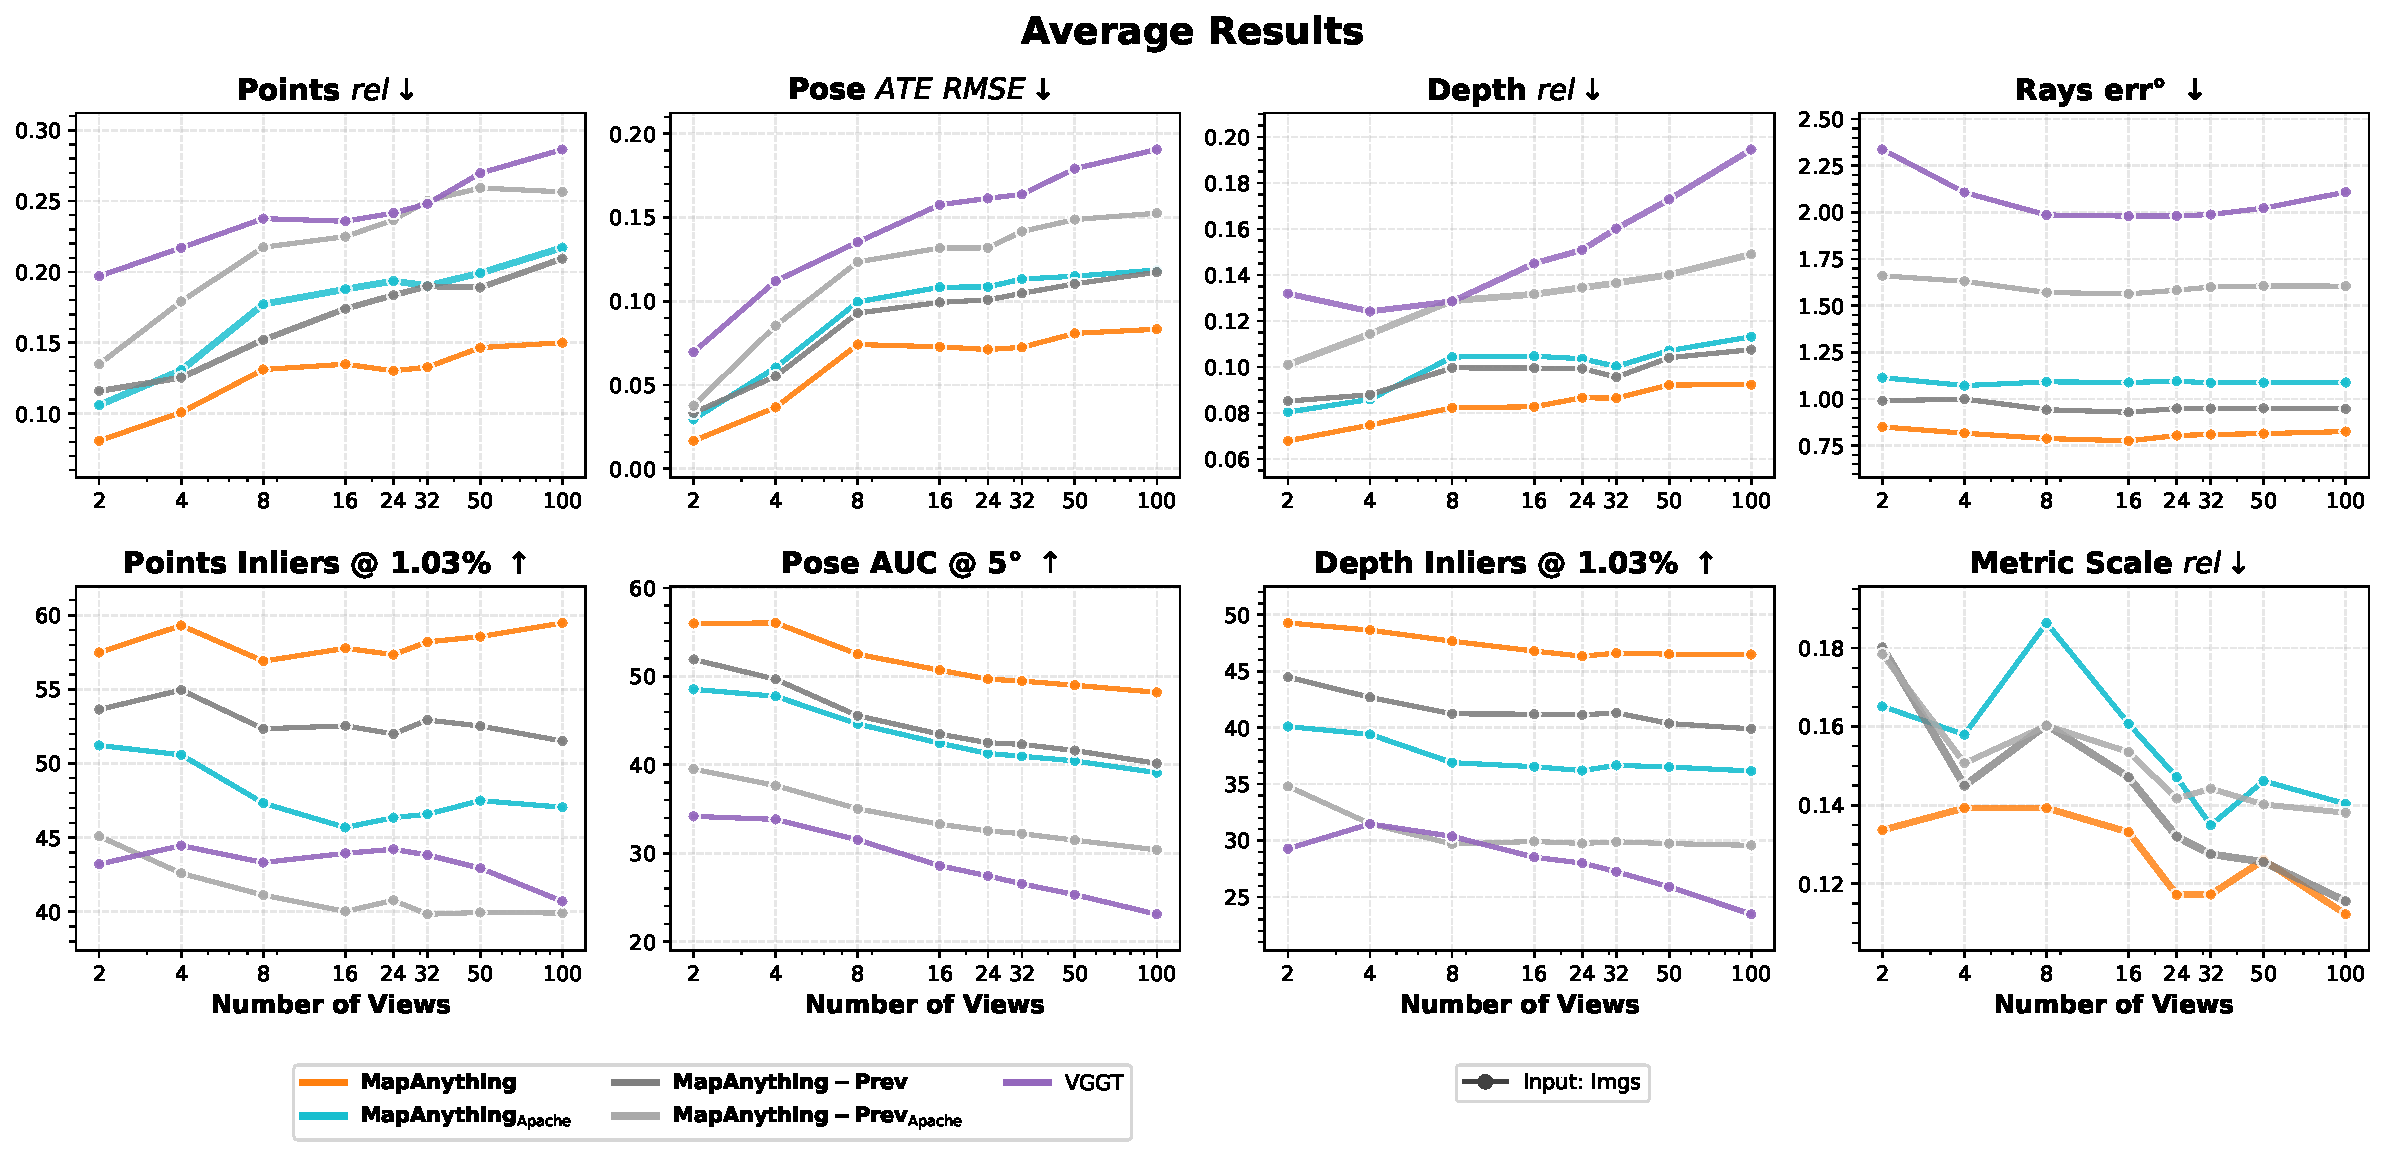
\includegraphics[trim={0cm 0cm 0cm 0.9cm},clip,width=\linewidth]{figs/V1_1_Benchmarking/v1_1_bench_present_vs_past/results_v1_1_bench_present_vs_past_average.pdf}

    \vspace{0.3em}
    
    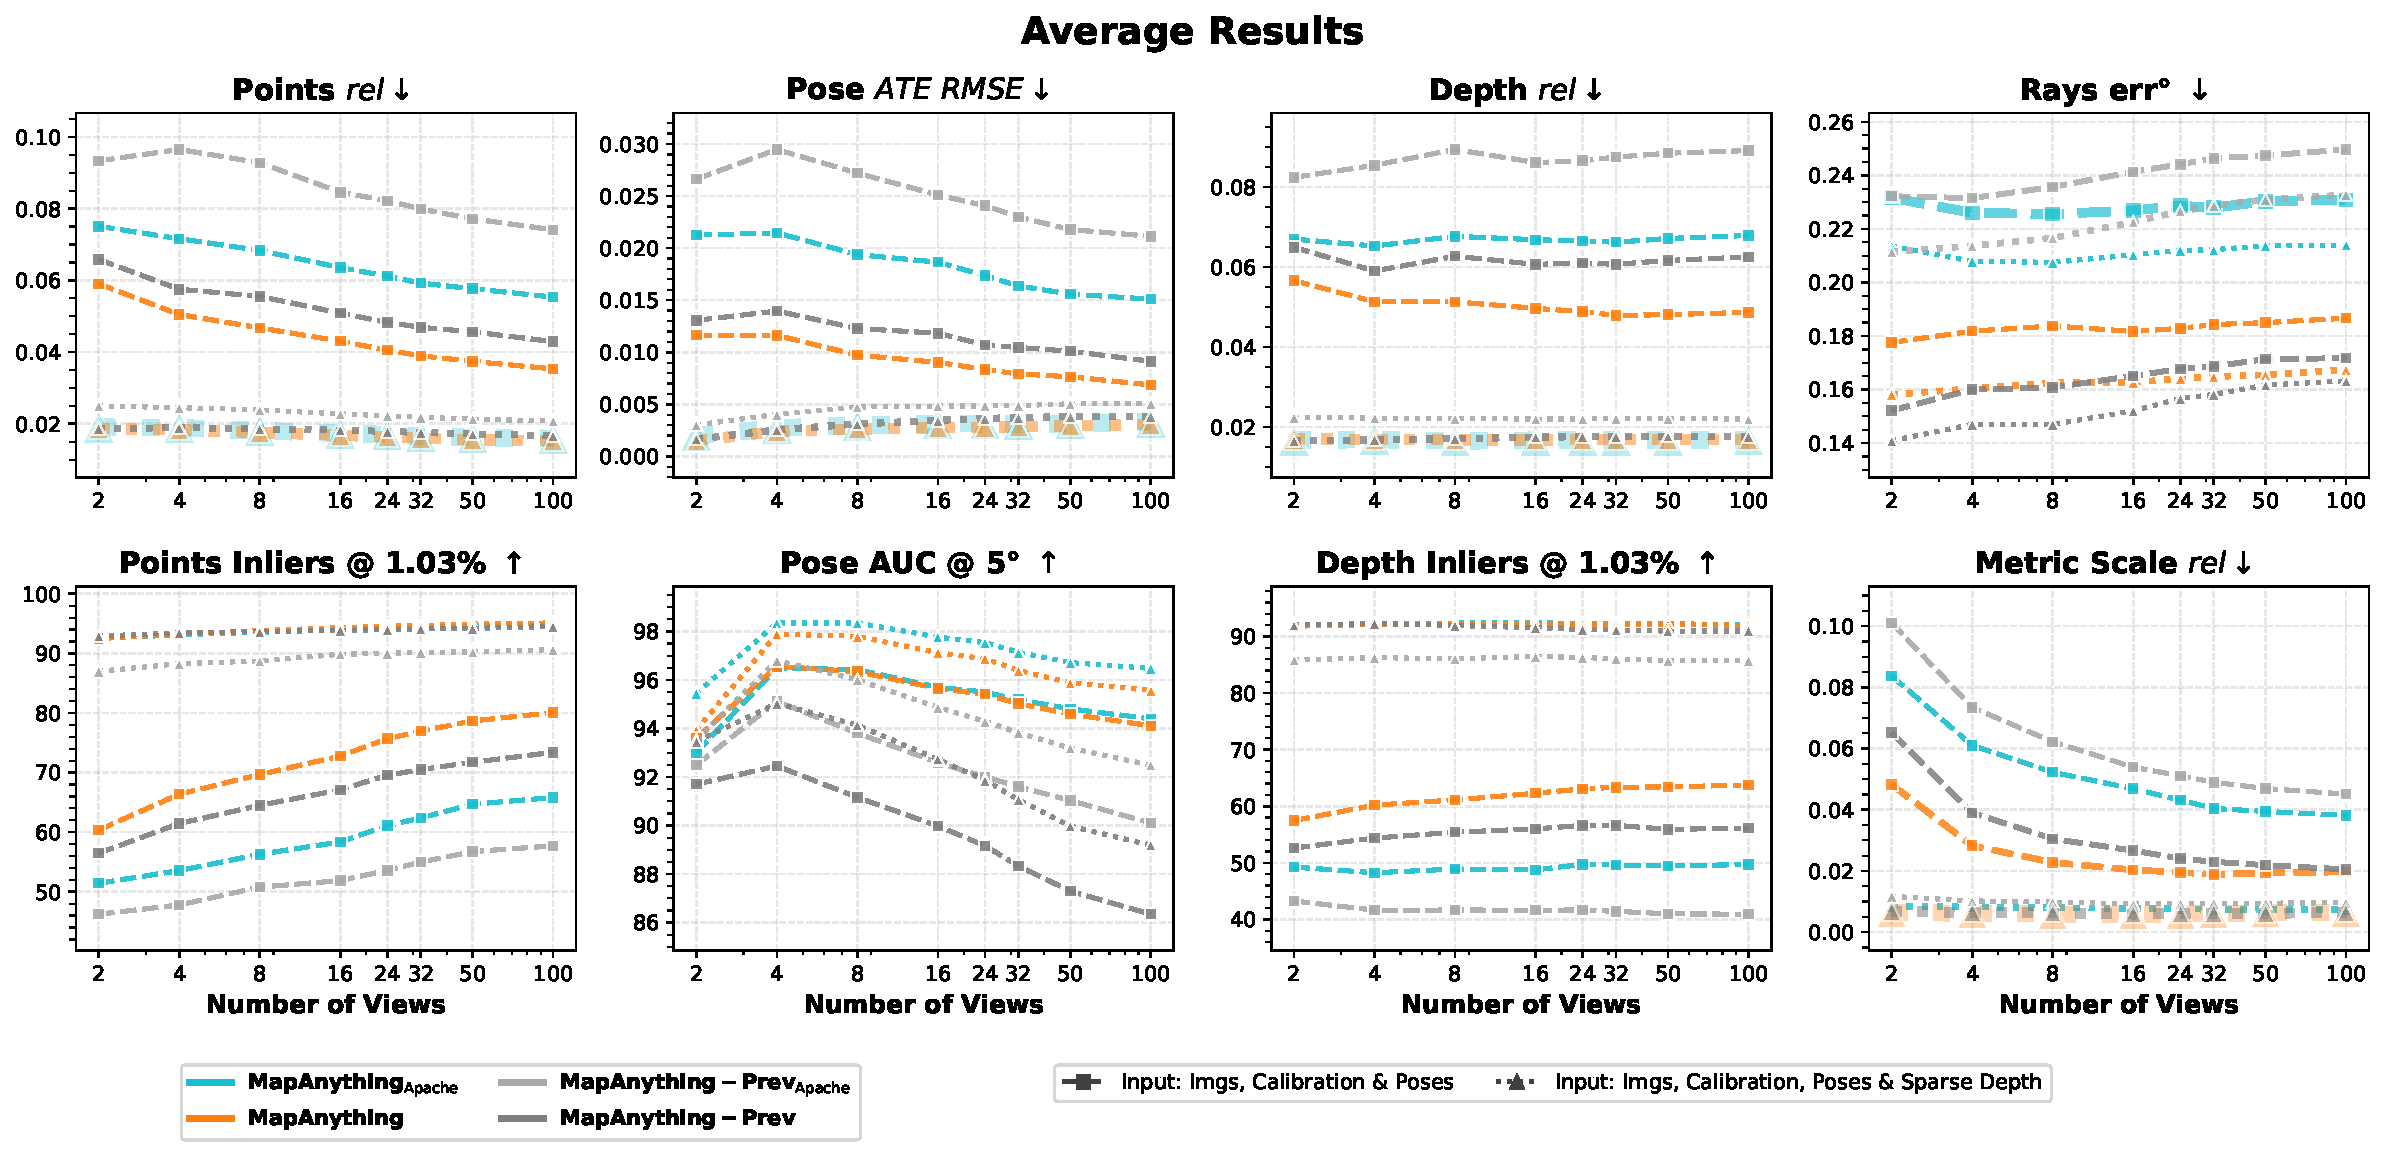
\includegraphics[trim={0cm 0cm 0cm 0.9cm},clip,width=\linewidth]{figs/V1_1_Benchmarking/v1_1_bench_multi_modal_present_vs_past/results_v1_1_bench_multi_modal_present_vs_past_average.pdf}
    
    \caption{\label{fig:v1_1_vs_v1}%
    \textbf{Dense multi-view reconstruction benchmarking comparing the performance of the latest checkpoint as of January 20th 2026 (\coolname) to the one released in September 2025 (\coolname-Prev).}
    The primary difference between the two variants (\textit{latest} \& \textit{previous}) is: (a) Encoder: First 24 layers of 1536-dim DINOv2 ViT-G (\textit{latest}) vs All 24 layers of 1024-dim DINOv2 ViT-L (\textit{previous}), (b) Multi-View Transformer: Last 16 layers of 1536-dim DINOv2 ViT-G (\textit{latest}) vs 24 layers of a randomly initialized 736-dim ViT-B size transformer.
    Both across large-scale trainings and ablation settings, we find that the DINOv2 initialization for the multi-view transformer helps significantly with convergence speed and final performance.
    In the above plots, we report the absolute relative error ($\absrel$), the inlier ratio at a relative threshold of $1.03\%$ ($\threshI$), the average aligned trajectory error ($ATE~RMSE$), the area under the curve at an error threshold of 5° ($AUC@5$), and the average angular error ($err$) in degrees (°), averaged over ETH3D, ScanNet++ v2 \& TAv2.
    }
\end{figure*}

\clearpage

\begin{figure*}[!ht]
    \centering
    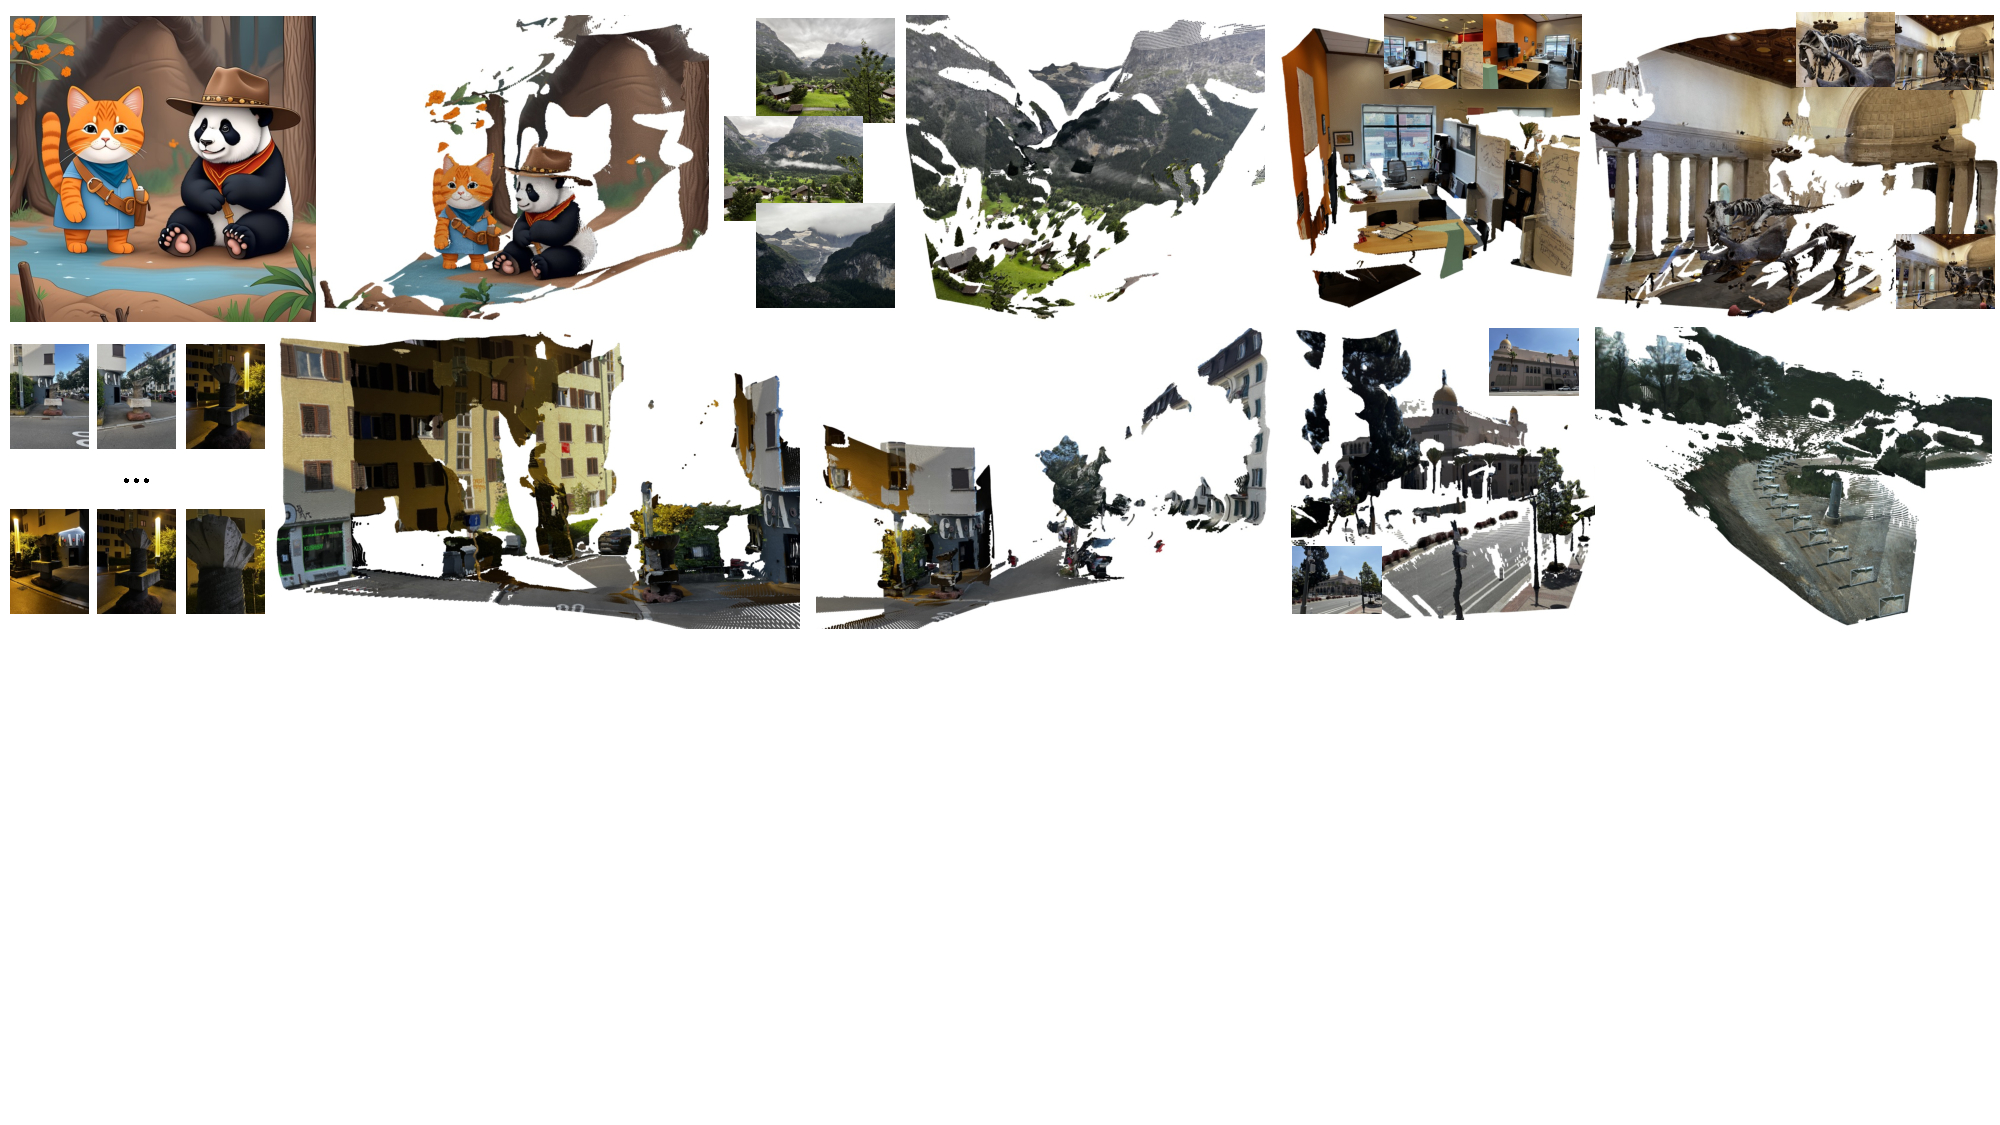
\includegraphics[trim={0cm 8cm 0cm 0cm},clip,width=\linewidth]{figs/Qual_Diversity_MapAnything.pdf}
    \caption{\textbf{\coolname provides high-fidelity dense geometric reconstructions} across varying domains and number of views. While \coolname can support a flexible set of inputs, here we are showcasing its capabilities only using images as input. In particular, we show results across a varying number of captured views and from different domains such as indoor, landscape, art, object-centric, and off-road. It also works well on monocular and art images despite not being trained for it.
}
    \label{fig:qual_diversity}
\end{figure*}

\begin{table*}[t]
    \centering
    \begin{minipage}{0.48\textwidth}
        \centering
        

\caption{\label{tab:supplementary_mapanything_input_variants}%
  \textbf{\coolname demonstrates remarkable flexibility in handling diverse input configurations, with performance improving as additional modalities are provided.}
  While our universal training supports 64 (i.e., $2^6$) possible input combinations, we highlight 12 representative combinations in this table.
  We report the absolute relative error ($\absrel$) and the inlier ratio at a relative threshold of 1.03\% ($\threshI$) for 50 views, averaged over ETH3D, ScanNet++ v2 \& TAv2.
  `K' denotes camera intrinsics and `sparse' depth indicates that 90\% of the valid depth is randomly masked out.
}
\centering
\scriptsize
\setlength{\tabcolsep}{1.5mm}
\begin{tabular}{cccccccccc}
\toprule
\multicolumn{7}{c}{\textbf{\coolname Inputs}}
& \multicolumn{3}{c}{\textbf{Avg. Performance}} \\
\cmidrule(lr){1-7} \cmidrule(lr){8-10}
& & & \multicolumn{2}{c}{\textbf{Depth}} & \multicolumn{2}{c}{\textbf{Metric Scale}}
& \textbf{Scale}
& \multicolumn{2}{c}{\textbf{Points}} \\
\textbf{Imgs} & \textbf{K} & \textbf{Poses}
& \textbf{Dense} & \textbf{Sparse} & \textbf{Pose} & \textbf{Depth}
& $\absrel\downarrow$
& $\absrel\downarrow$ & $\threshI\uparrow$
\\
\midrule
\multicolumn{10}{l}{\textbf{a) Images Only}} \\[0.4em]
\greencheck & \redx & \redx & \redx & \redx & \redx & \redx         
  & 0.13   
  & 0.15           
  & 58.6       
  \\

\arrayrulecolor{lightgray}\midrule
\multicolumn{10}{l}{\textbf{b) Images \& Intrinsics}} \\[0.4em]
\greencheck & \greencheck & \redx & \redx & \redx & \redx & \redx         
  & 0.13   
  & 0.14           
  & 61.5       
  \\

\arrayrulecolor{lightgray}\midrule
\multicolumn{10}{l}{\textbf{c) Images \& Poses}} \\[0.4em]
\greencheck & \redx & \greencheck & \redx & \redx & \redx & \redx         
  & 0.11   
  & 0.04           
  & 76.8       
  \\
\greencheck & \redx & \greencheck & \redx & \redx & \greencheck & \redx         
  & 0.02   
  & 0.04           
  & 75.3       
  \\

\arrayrulecolor{lightgray}\midrule
\multicolumn{10}{l}{\textbf{d) Images, Intrinsics \& Poses}} \\[0.4em]
\greencheck & \greencheck & \greencheck & \redx & \redx & \redx & \redx         
  & 0.11   
  & 0.03           
  & 80.5       
  \\
\greencheck & \greencheck & \greencheck & \redx & \redx & \greencheck & \redx         
  & 0.02   
  & 0.04           
  & 78.7       
  \\

\arrayrulecolor{lightgray}\midrule
\multicolumn{10}{l}{\textbf{e) Images \& Depth}} \\[0.4em]
\greencheck & \greencheck & \redx & \redx & \greencheck & \redx & \greencheck         
  & 0.04   
  & 0.11           
  & 77.2       
  \\
\greencheck & \greencheck & \redx & \greencheck & \redx & \redx & \greencheck         
  & 0.05   
  & 0.11           
  & 67.8       
  \\

\arrayrulecolor{lightgray}\midrule
\multicolumn{10}{l}{\textbf{f) Images, Intrinsics, Poses \& Depth}} \\[0.4em]
\greencheck & \greencheck & \greencheck & \redx & \greencheck & \redx & \redx         
  & 0.12   
  & 0.02           
  & 92.0       
  \\
\greencheck & \greencheck & \greencheck & \greencheck & \redx & \redx & \redx         
  & 0.12   
  & 0.02           
  & 83.0       
  \\
\greencheck & \greencheck & \greencheck & \redx & \greencheck & \greencheck & \greencheck         
  & 0.01   
  & 0.02           
  & 94.9       
  \\
\greencheck & \greencheck & \greencheck & \greencheck & \redx & \greencheck & \greencheck         
  & 0.01   
  & 0.02           
  & 84.4       
  \\

\arrayrulecolor{black}\bottomrule
\end{tabular}



































    \end{minipage}
    \hfill %
    \begin{minipage}{0.48\textwidth}
        \centering
          \centering
  \caption{\label{tab:ablations_loss_attention}%
    \textbf{Ablations showing loss and multi-view transformer attention design choices critical for strong reconstruction performance.} %
    We report the absolute relative error ($\absrel$) and the inlier ratio at a relative threshold of 1.03\% ($\threshI$) at 50 views, averaged over ETH3D, ScanNet++ v2 \& TAv2.
    Best results are \textbf{bold}.
  }
  \begin{subtable}[t]{0.49\linewidth}
    \centering
    \caption{\textbf{Loss Scheme}}
    \resizebox{\textwidth}{!}{
\begin{tabular}{l|c|cc|}
\toprule
    & \multicolumn{3}{c|}{\textbf{ETH3D, SN++v2 \& TAV2}}

    \\

    \cmidrule(lr){2-4} 

    & \textbf{Metric Scale} & \multicolumn{2}{c|}{\textbf{Pointmaps}}

    \\

    \cmidrule(lr){2-2} \cmidrule(lr){3-4}

    \textbf{Methods}
    & $\absrel\downarrow$
    & $\absrel\downarrow$ & $\threshI\uparrow$

    \\

    \midrule

    \multicolumn{4}{l}{\textbf{Input: Images Only}}
    \\

    \emph{Overall Factored Loss}
    & \textbf{0.16}
    & \textbf{0.29}
    & \textbf{31.8}
    \\

    No Log Loss
    & 0.17
    & 0.39
    & 27.3
    \\

\bottomrule
\end{tabular}
}

    \label{tab:ablation_loss}
  \end{subtable}%
  \hfill
  \begin{subtable}[t]{0.50\linewidth}
    \centering
    \caption{\textbf{Attention Scheme}}
    \resizebox{\textwidth}{!}{
\begin{tabular}{l|c|cc|}
\toprule
    & \multicolumn{3}{c|}{\textbf{ETH3D, SN++v2 \& TAV2}}

    \\

    \cmidrule(lr){2-4} 

    & \textbf{Metric Scale} & \multicolumn{2}{c|}{\textbf{Pointmaps}}

    \\

    \cmidrule(lr){2-2} \cmidrule(lr){3-4}

    \textbf{Methods}
    & $\absrel\downarrow$
    & $\absrel\downarrow$ & $\threshI\uparrow$

    \\

    \midrule

    \multicolumn{4}{l}{\textbf{Input: Images Only}}
    \\

    \emph{Alternating}~\cite{WangCKVRN2025}
    & \textbf{0.16}
    & \textbf{0.29}
    & \textbf{31.8}
    \\

    Global w/ View PE~\cite{YangSLHTCCMF2025}
    & 0.20
    & 0.53
    & 19.7
    \\

\bottomrule
\end{tabular}
}

    \label{tab:ablation_attention}
  \end{subtable}%

    \end{minipage}
\end{table*}



\clearpage

\begin{figure*}[!t]
    \centering
    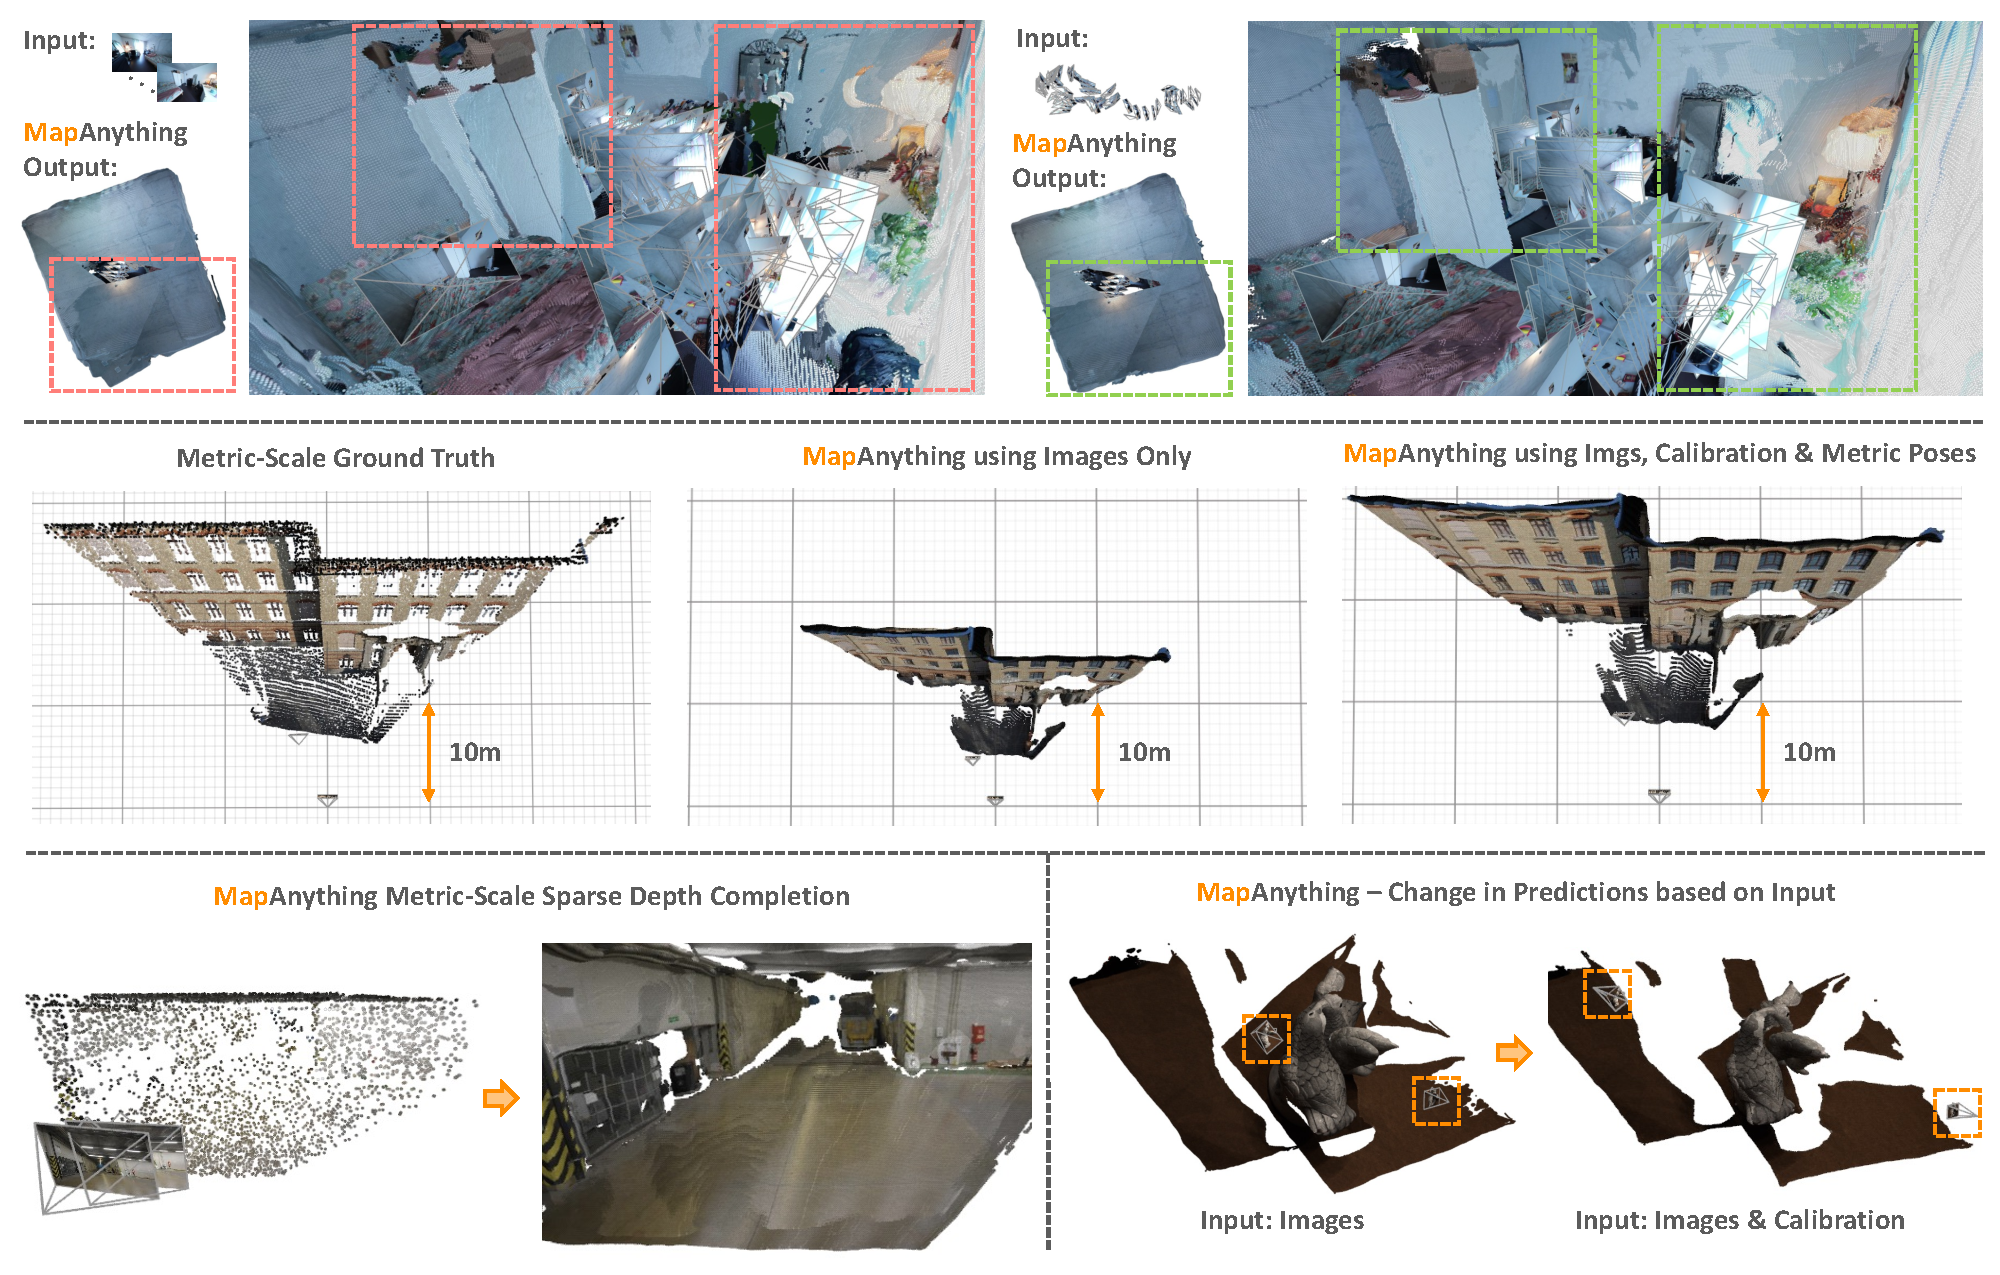
\includegraphics[width=0.9\linewidth]{figs/MapAnything_Geometric_Input_Benefits.pdf}
    \caption{\textbf{Auxiliary geometric inputs improve feed-forward performance of \coolname.} \texttt{(Top)} While \coolname \& other baselines using 100 input images show duplication of 3D structure, when provided with the camera calibration and poses, the 3D reconstruction significantly improves, showing aligned geometry. \texttt{(Middle)} \coolname using images only as input shows non-precise metric scale estimation on ETH3D (a zero-shot dataset). However, when the calibration and metric poses are provided as additional input, the estimated metric scale significantly improves and approximately matches the ground truth. \texttt{(Bottom-Left)} We show that \coolname can leverage a sparse metric point cloud as input to perform dense metric depth completion. \texttt{(Bottom-Right)} Despite not being trained for object-centric data, we show how the scene geometry and cameras change based on the input provided.
    }
    \label{fig:qual_geometric_inputs}
\end{figure*}

\clearpage

\begin{figure*}[!t]
    \centering

    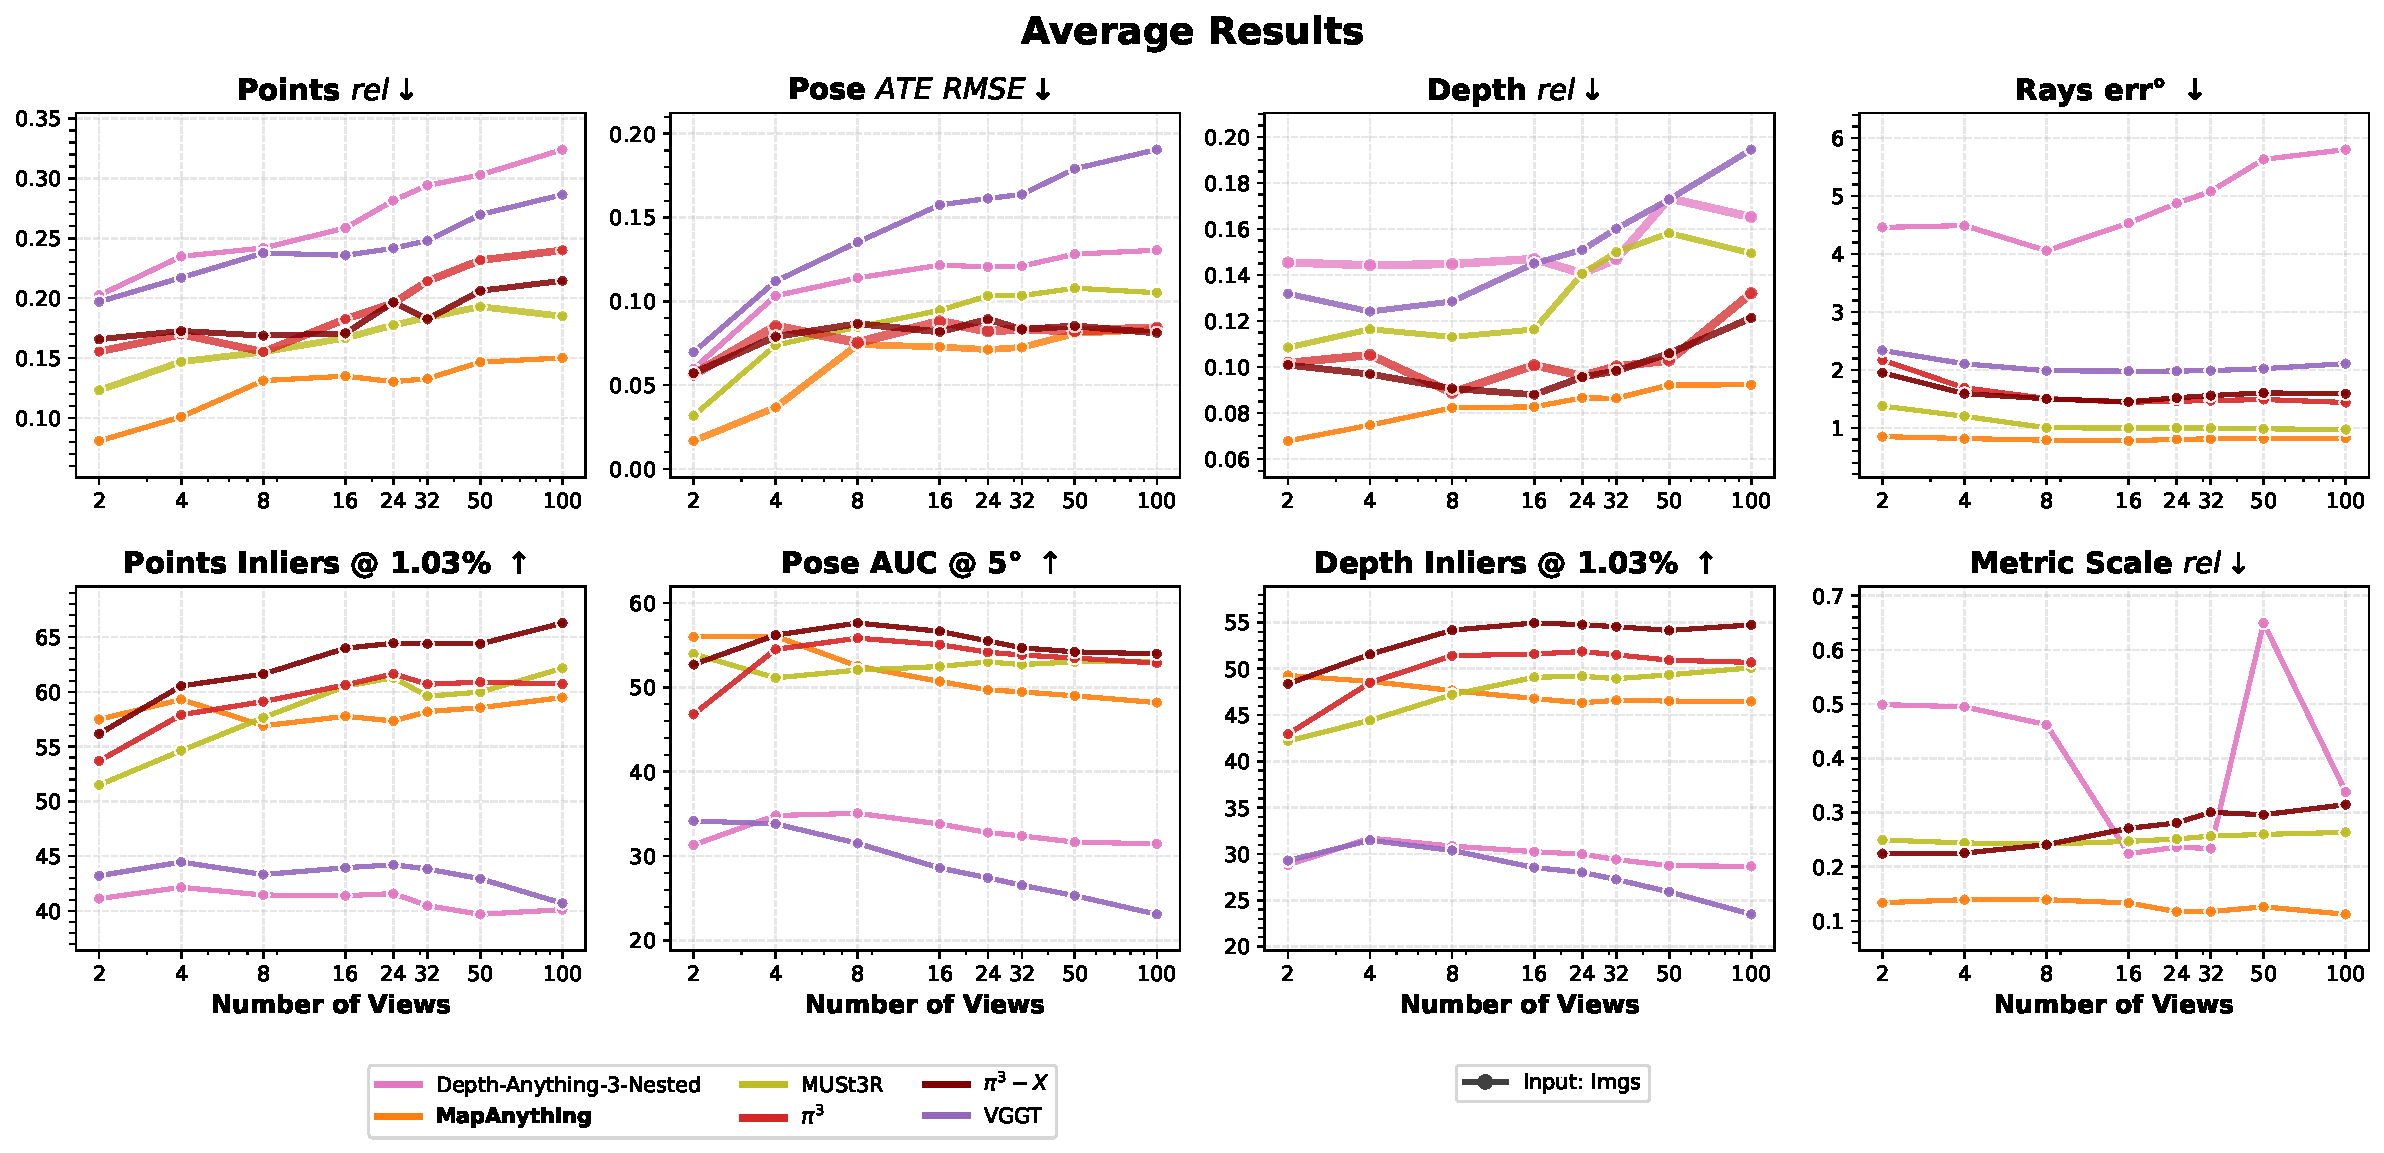
\includegraphics[trim={0cm 0cm 0cm 0cm},clip,width=\linewidth]{figs/V1_1_Benchmarking/v1_1_bench_latest_image_only/results_v1_1_bench_latest_image_only_average.pdf}

    \vspace{0.3em}
    
    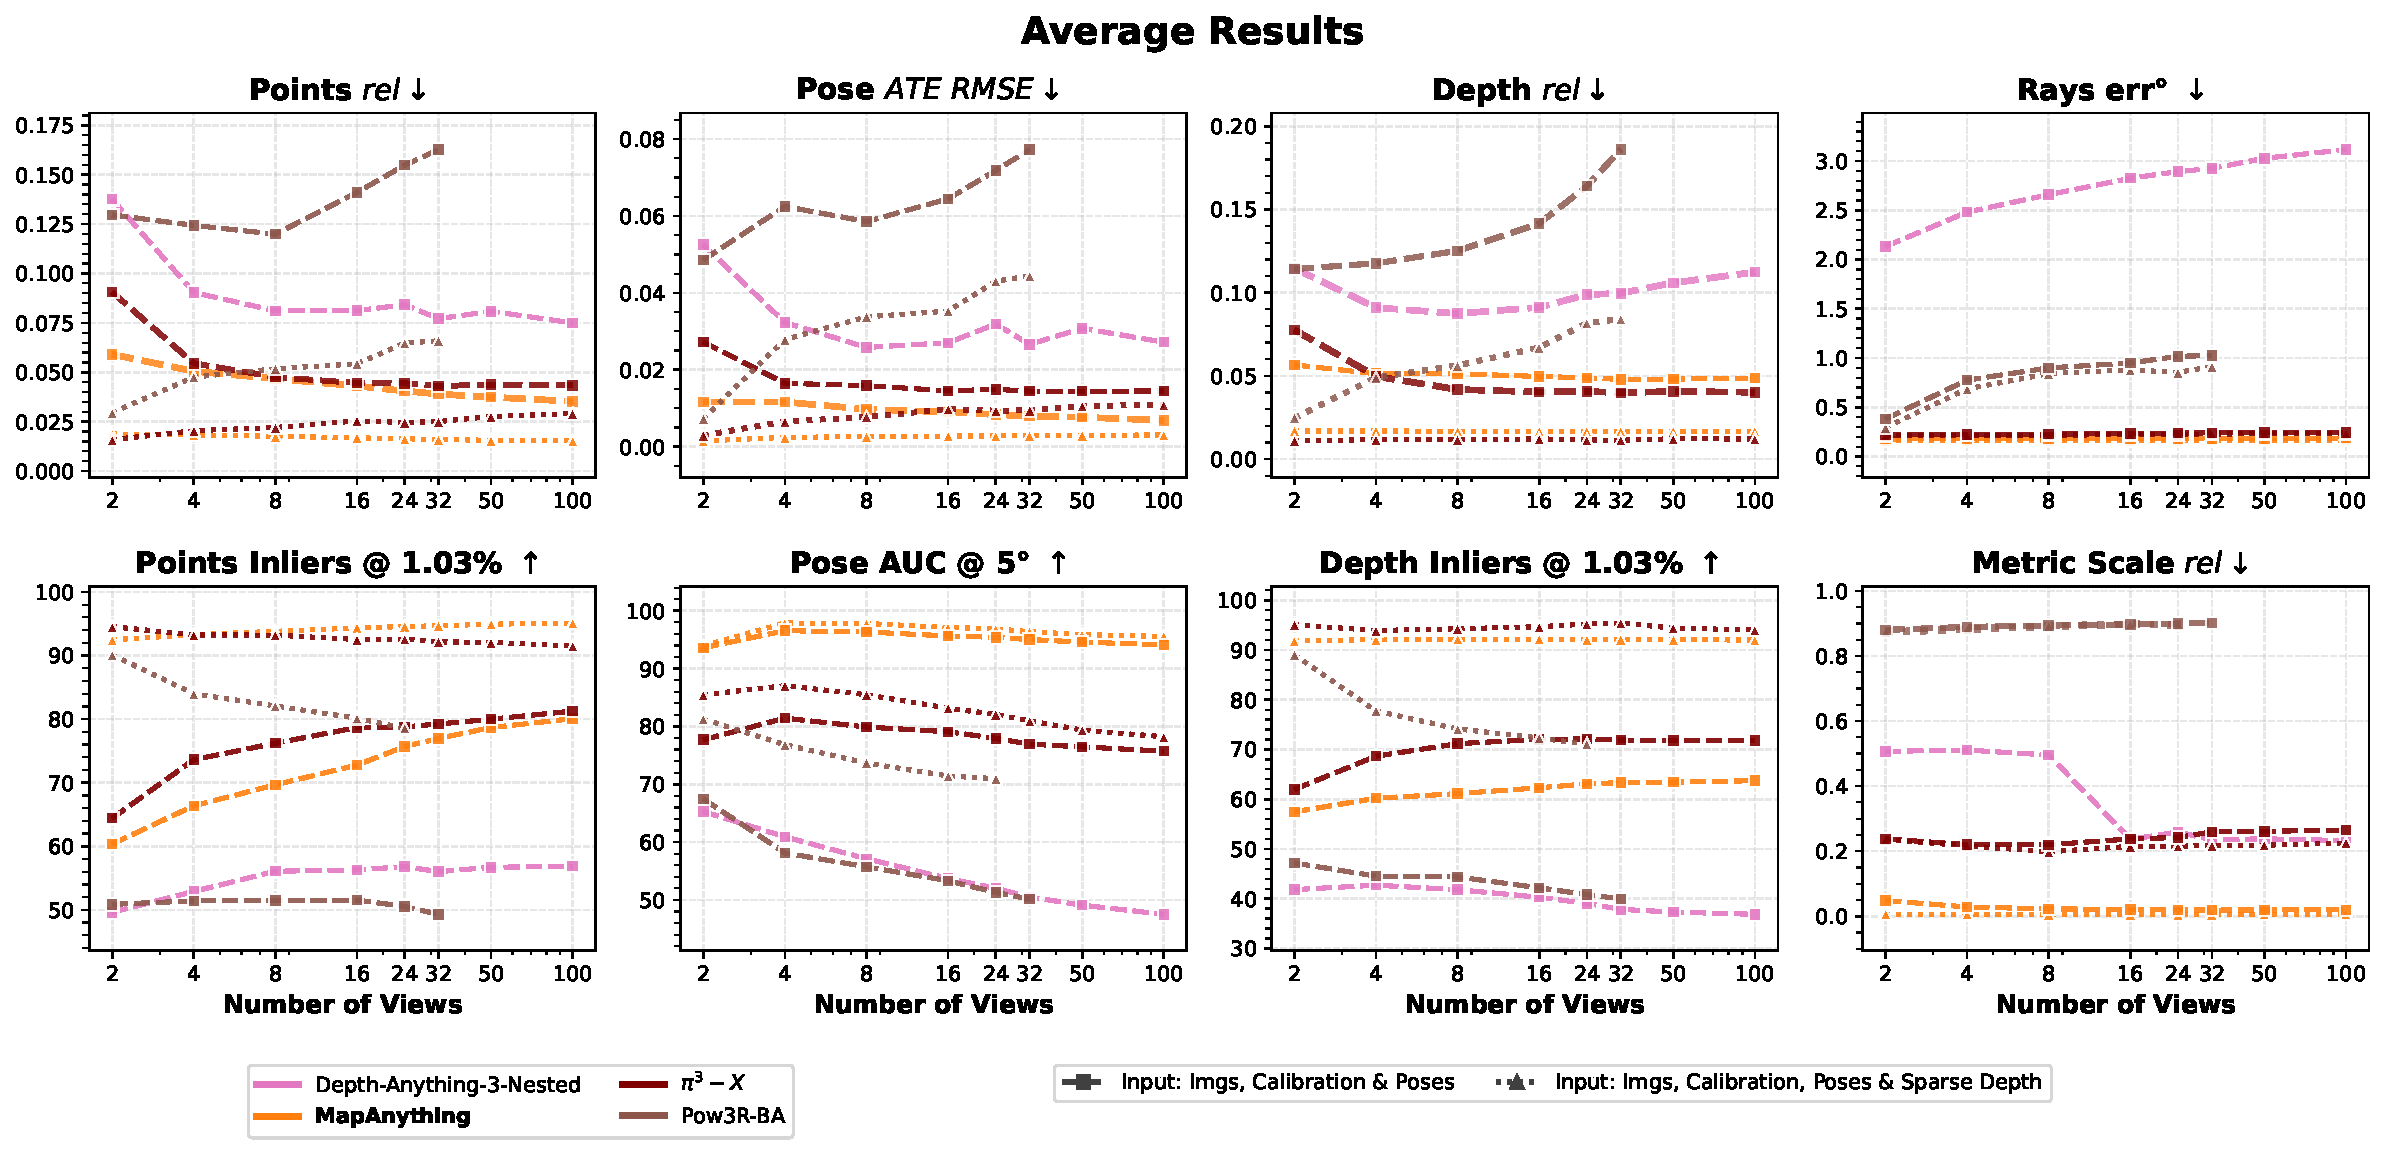
\includegraphics[trim={0cm 0cm 0cm 0cm},clip,width=\linewidth]{figs/V1_1_Benchmarking/v1_1_bench_latest_multi_modal/results_v1_1_bench_latest_multi_modal_average.pdf}
    
    \caption{\label{fig:v1_1_bench_average}%
    \textbf{\coolname showcases state-of-the-art and competitive dense multi-view reconstruction performance in comparison to latest public concurrent state-of-the-art models as of January 20th 2026, i.e., DA3-Nested \& $\pi^3$-X, despite being trained on significantly less amount of data.}
    We report the absolute relative error ($\absrel$), the inlier ratio at a relative threshold of $1.03\%$ ($\threshI$), the average aligned trajectory error ($ATE~RMSE$), the area under the curve at an error threshold of 5° ($AUC@5$), and the average angular error ($err$) in degrees (°), averaged over ETH3D, ScanNet++ v2 \& TAv2.
    }
\end{figure*}

\clearpage

\begin{figure*}[!t]
    \centering

    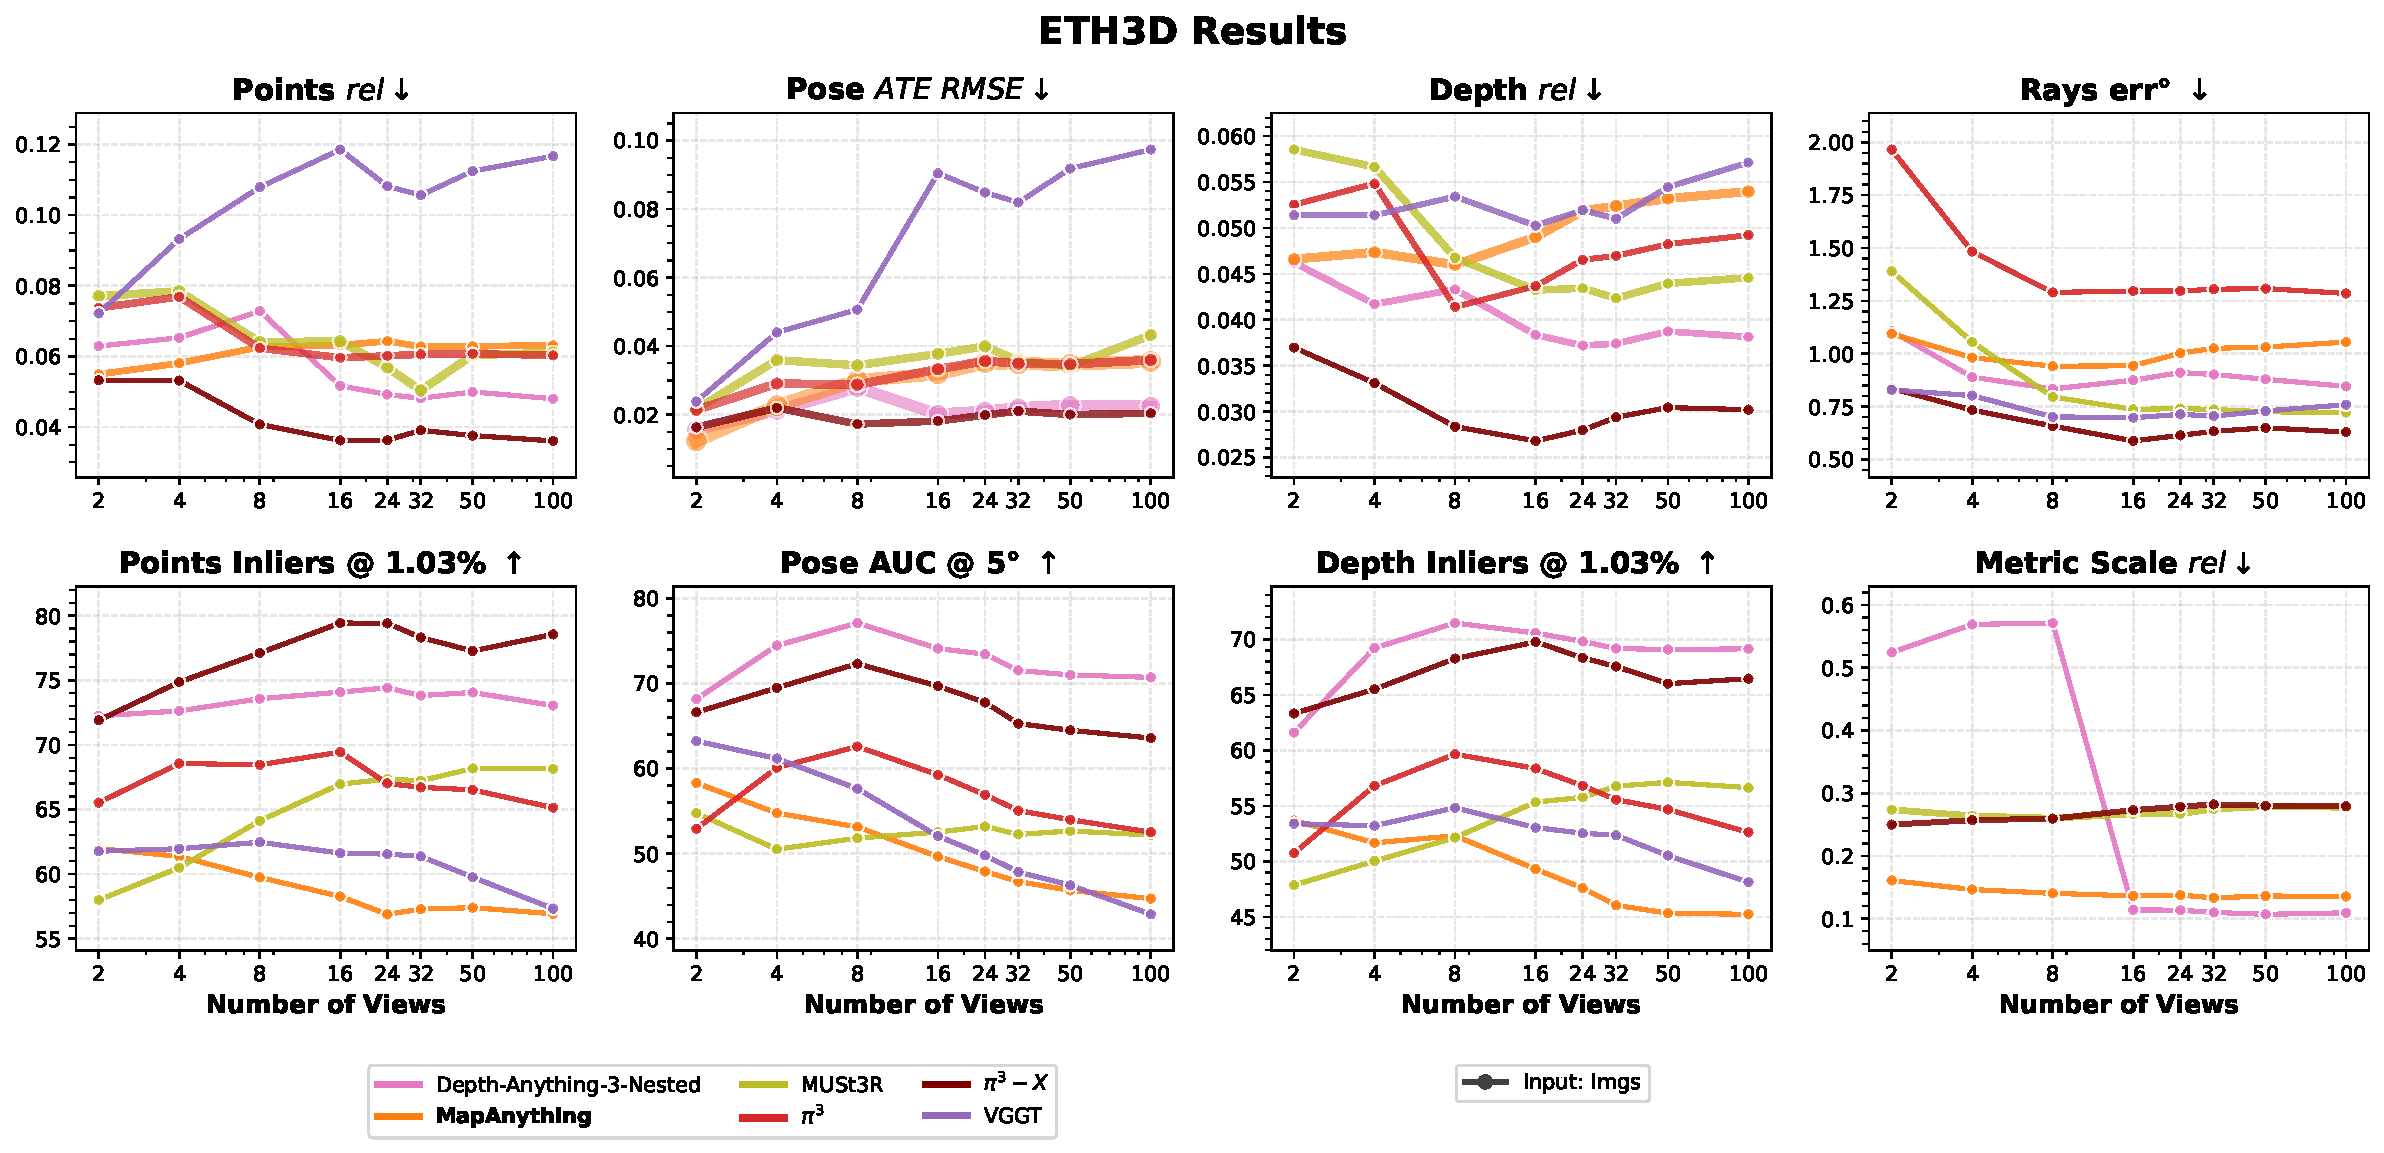
\includegraphics[trim={0cm 2cm 0cm 0cm},clip,width=0.9\linewidth]{figs/V1_1_Benchmarking/v1_1_bench_latest_image_only/results_v1_1_bench_latest_image_only_eth3d.pdf}

    \vspace{0.3em}
    
    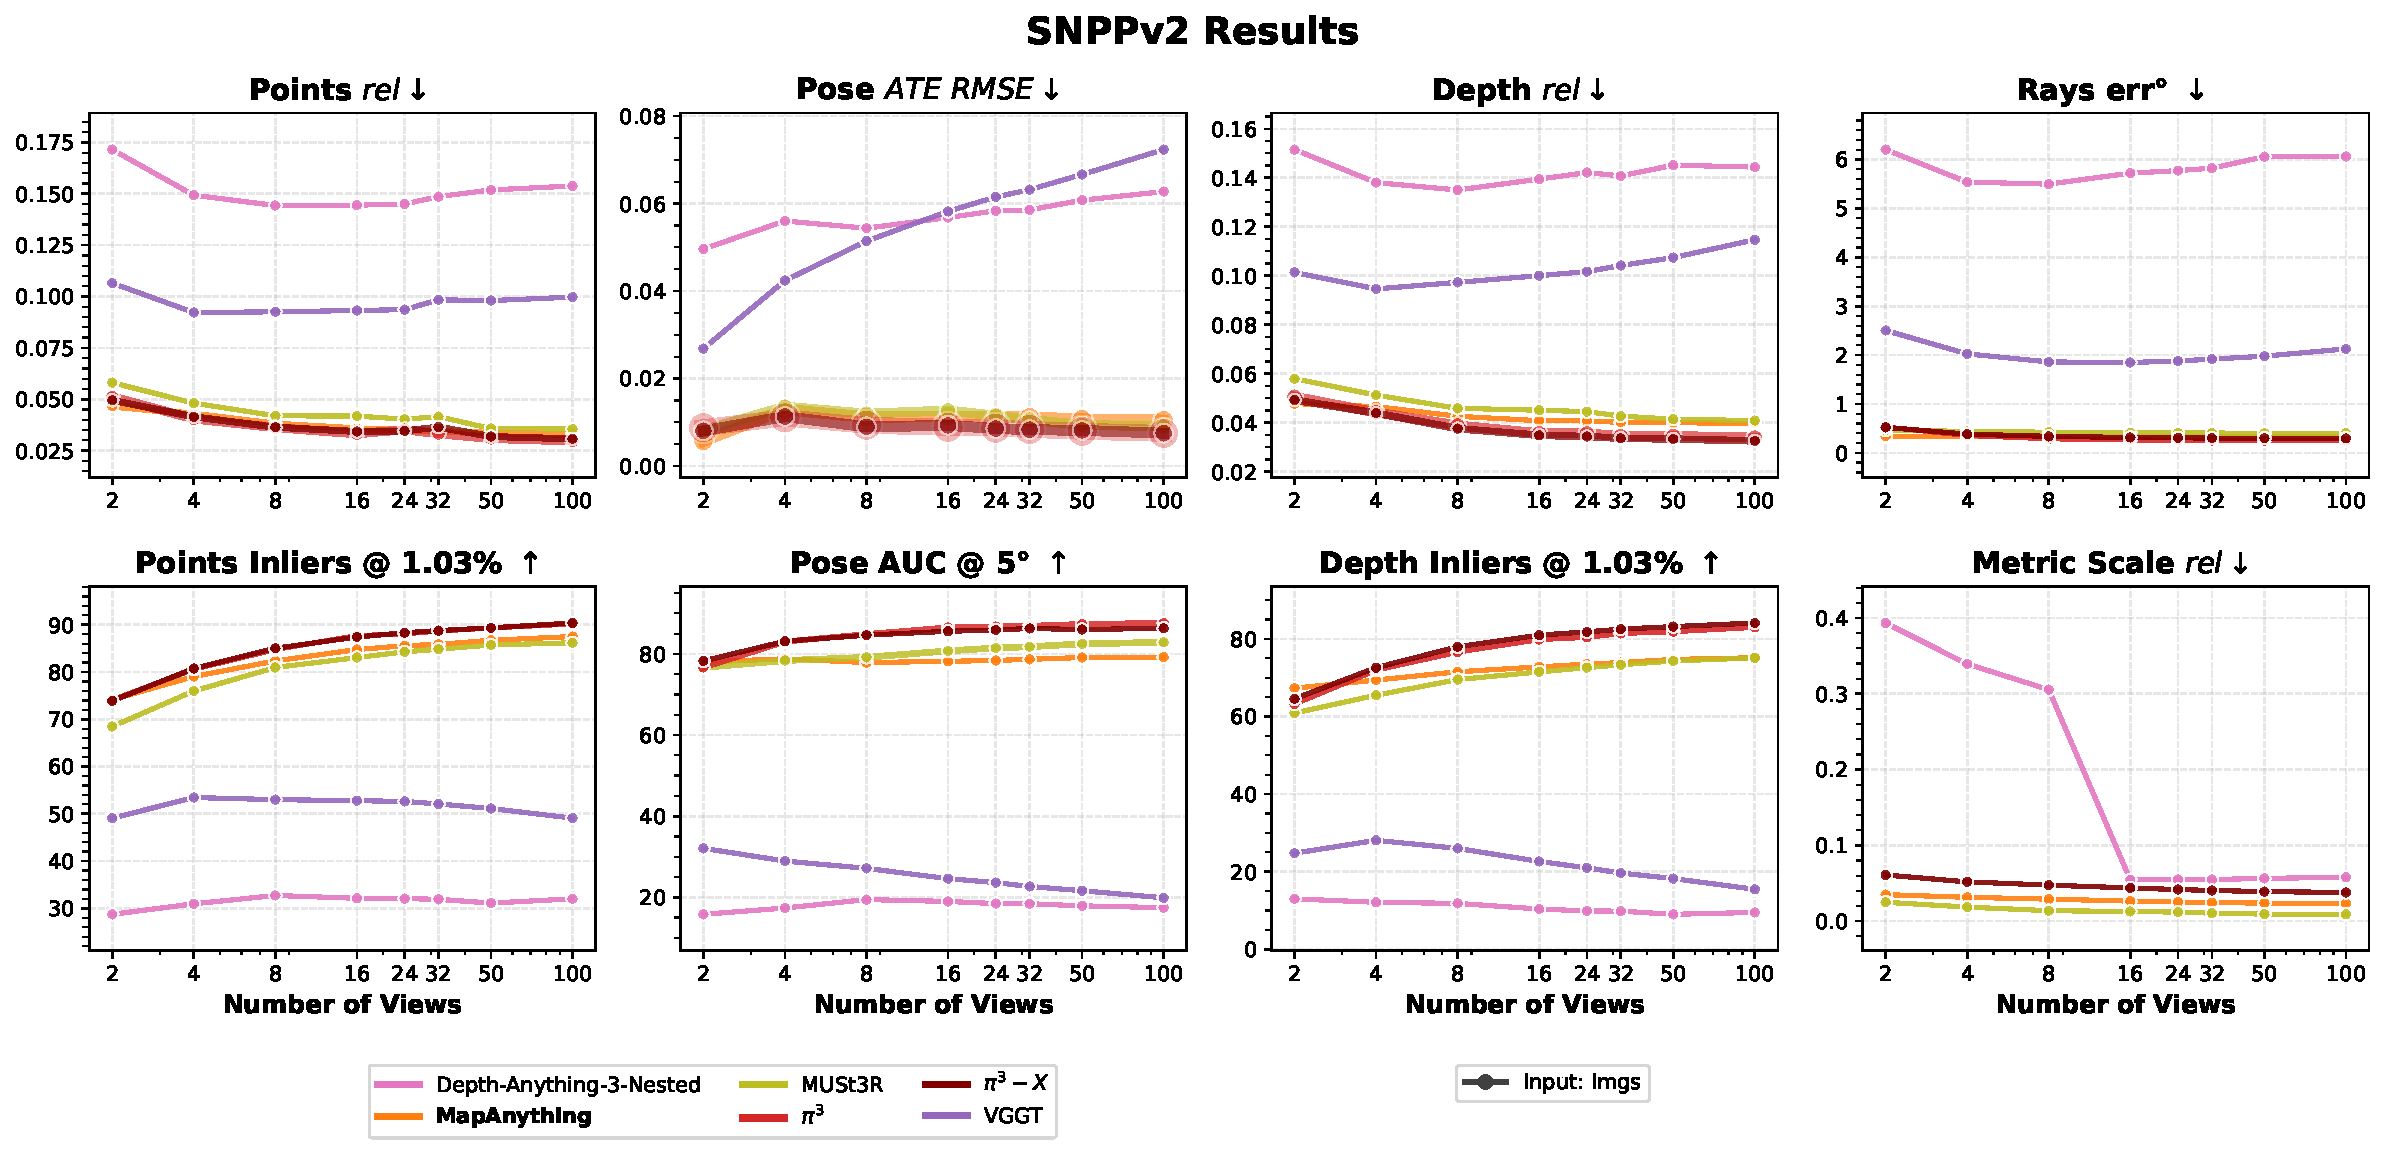
\includegraphics[trim={0cm 2cm 0cm 0cm},clip,width=0.9\linewidth]{figs/V1_1_Benchmarking/v1_1_bench_latest_image_only/results_v1_1_bench_latest_image_only_snppv2.pdf}

    \vspace{0.3em}
    
    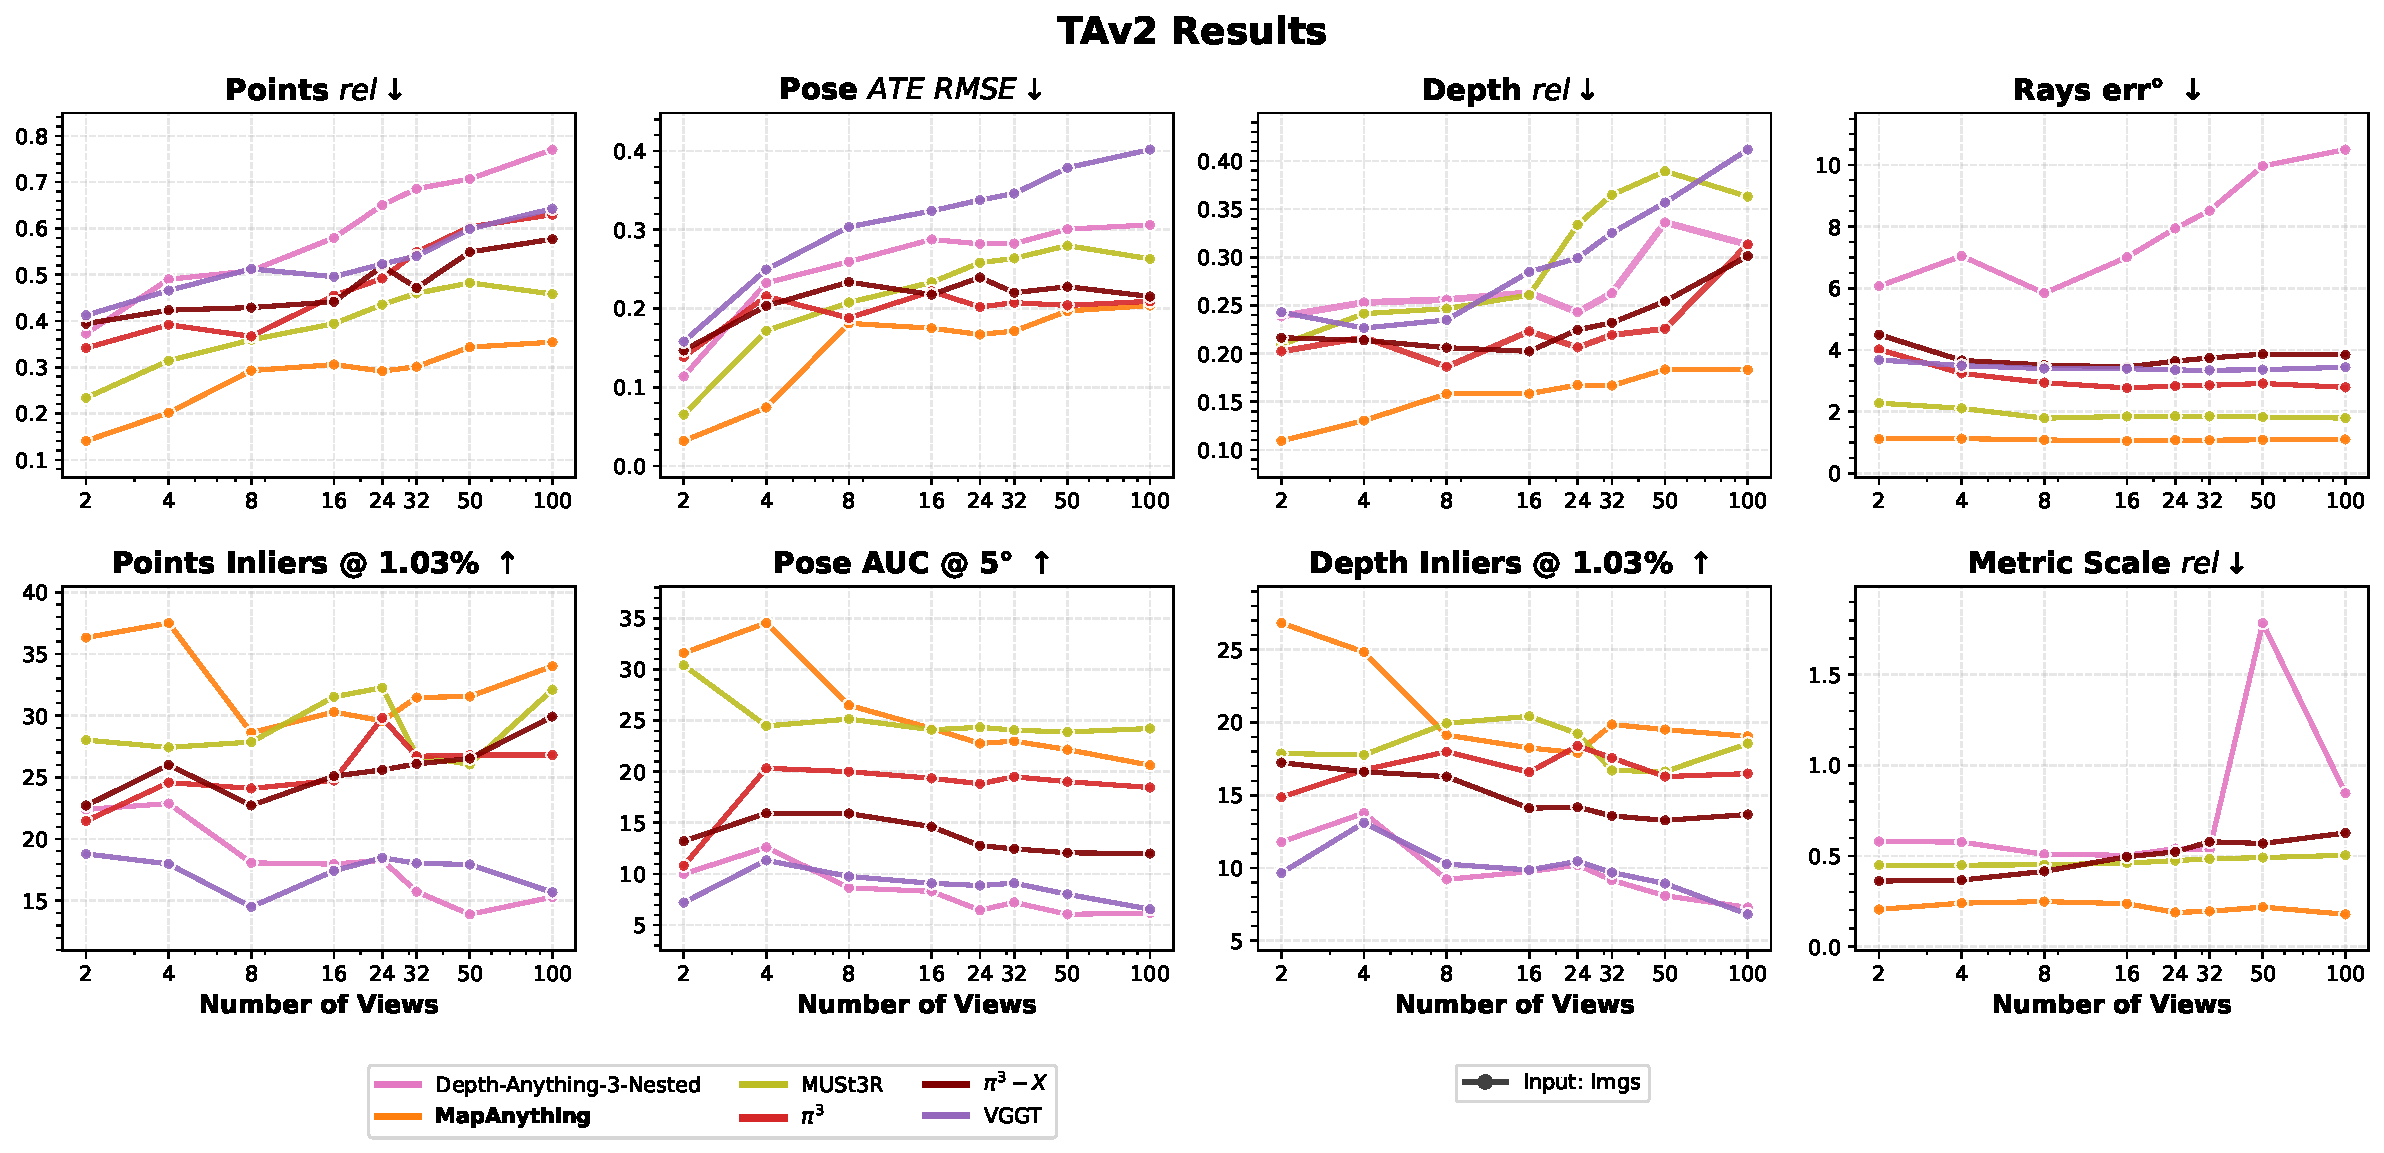
\includegraphics[trim={0cm 0cm 0cm 0cm},clip,width=0.9\linewidth]{figs/V1_1_Benchmarking/v1_1_bench_latest_image_only/results_v1_1_bench_latest_image_only_tav2.pdf}
    
    \caption{\label{fig:v1_1_bench_img_only_per_dataset}%
    \textbf{Dense multi-view reconstruction benchmarking across individual datasets using only images as input.}
    We also include results for latest public concurrent state-of-the-art models as of January 20th 2026.
    Please see \cref{fig:v1_1_bench_average} for details \& the averaged version.
    }
\end{figure*}

\clearpage

\begin{figure*}[!t]
    \centering

    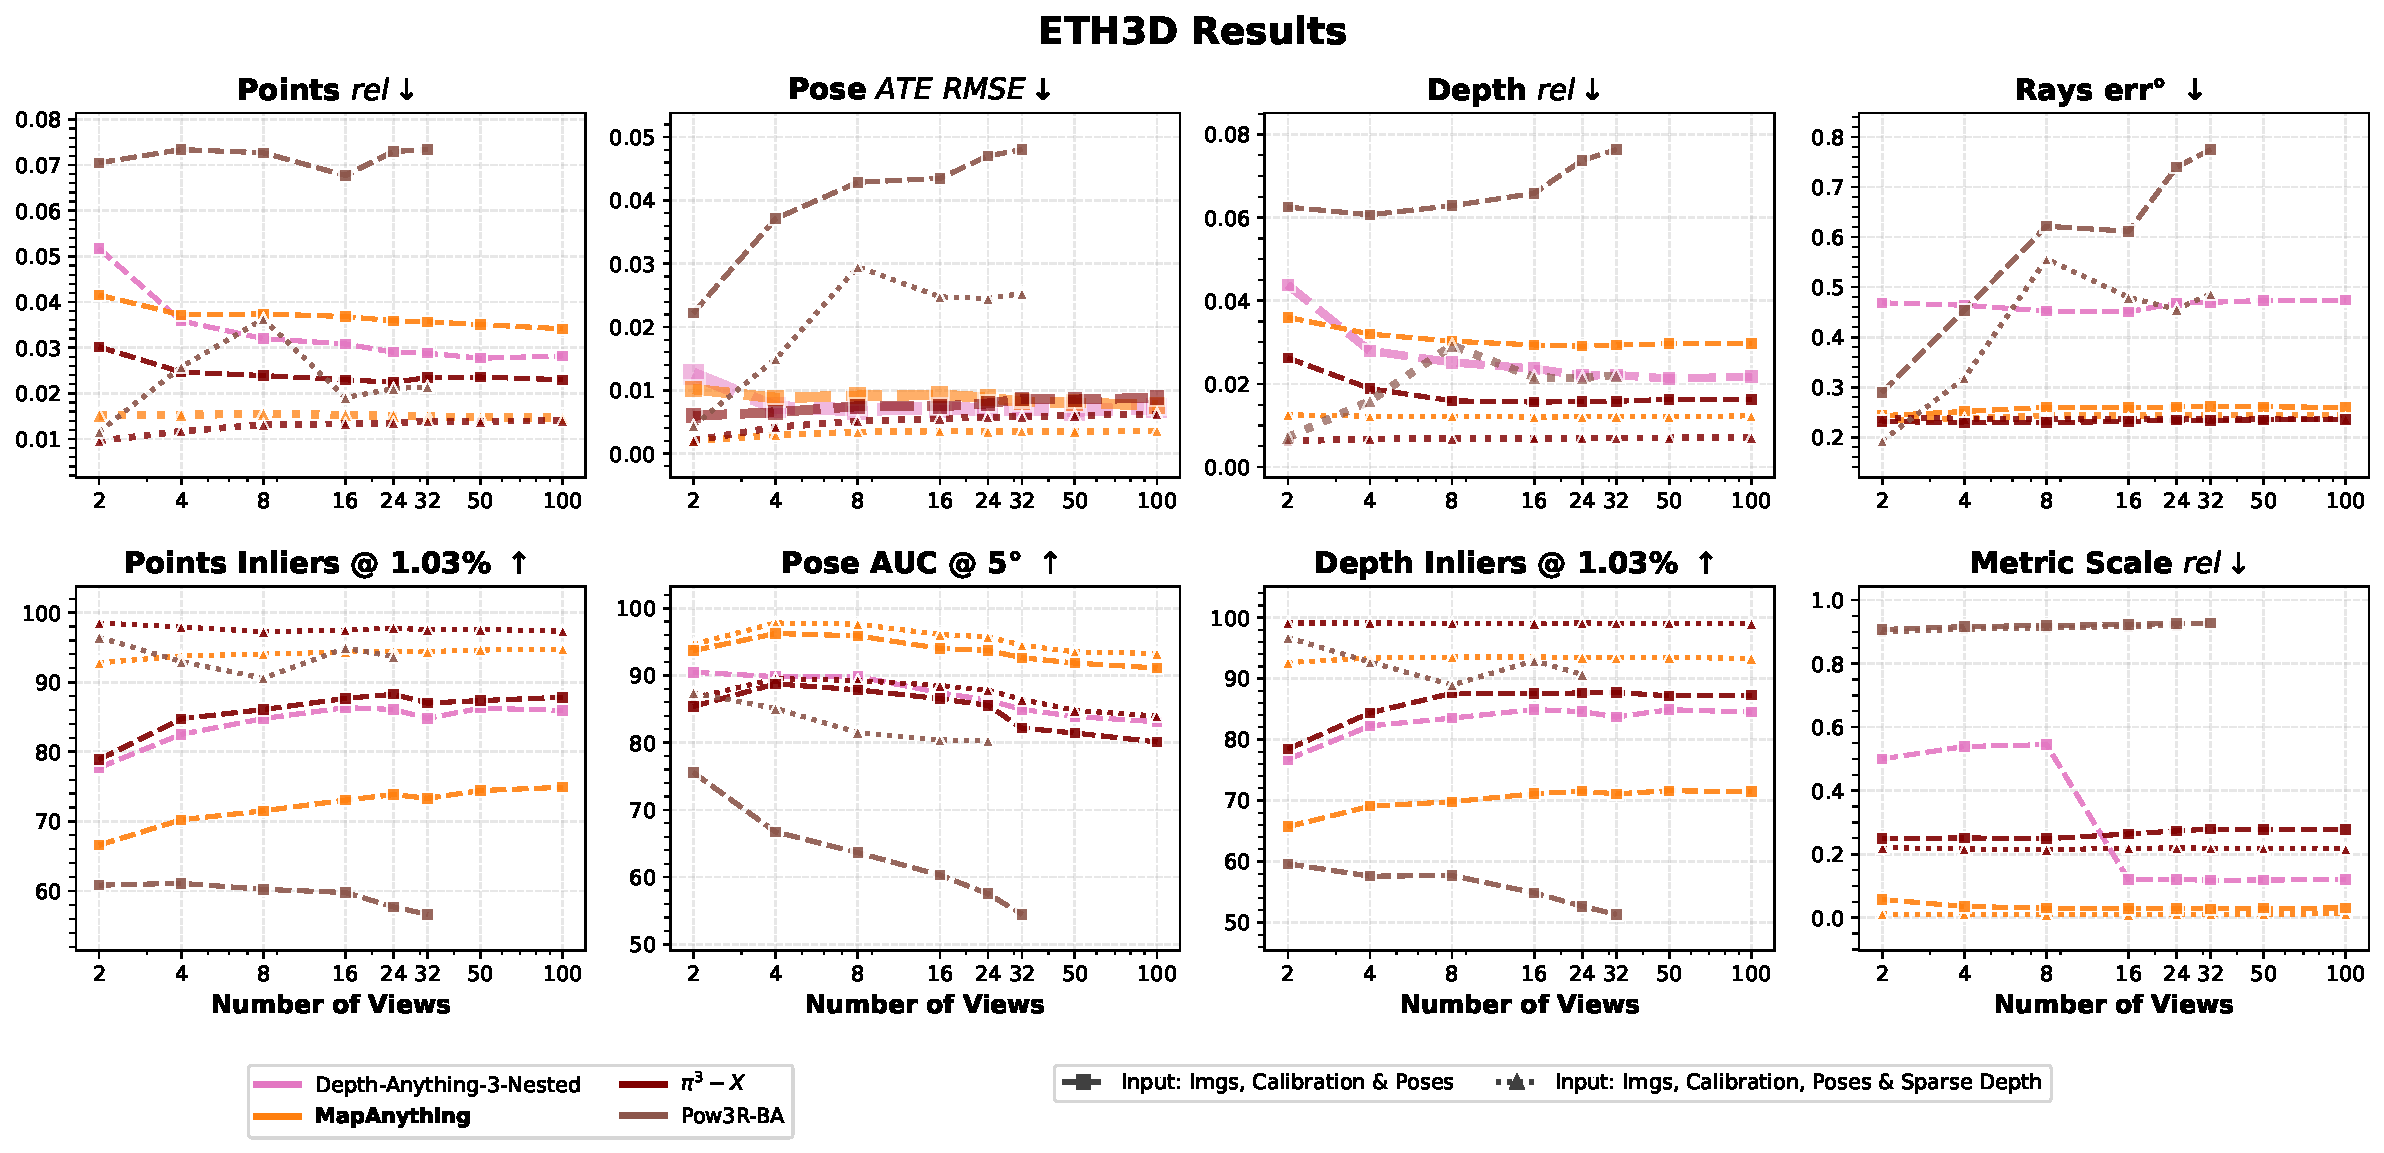
\includegraphics[trim={0cm 2cm 0cm 0cm},clip,width=0.9\linewidth]{figs/V1_1_Benchmarking/v1_1_bench_latest_multi_modal/results_v1_1_bench_latest_multi_modal_eth3d.pdf}

    \vspace{0.3em}
    
    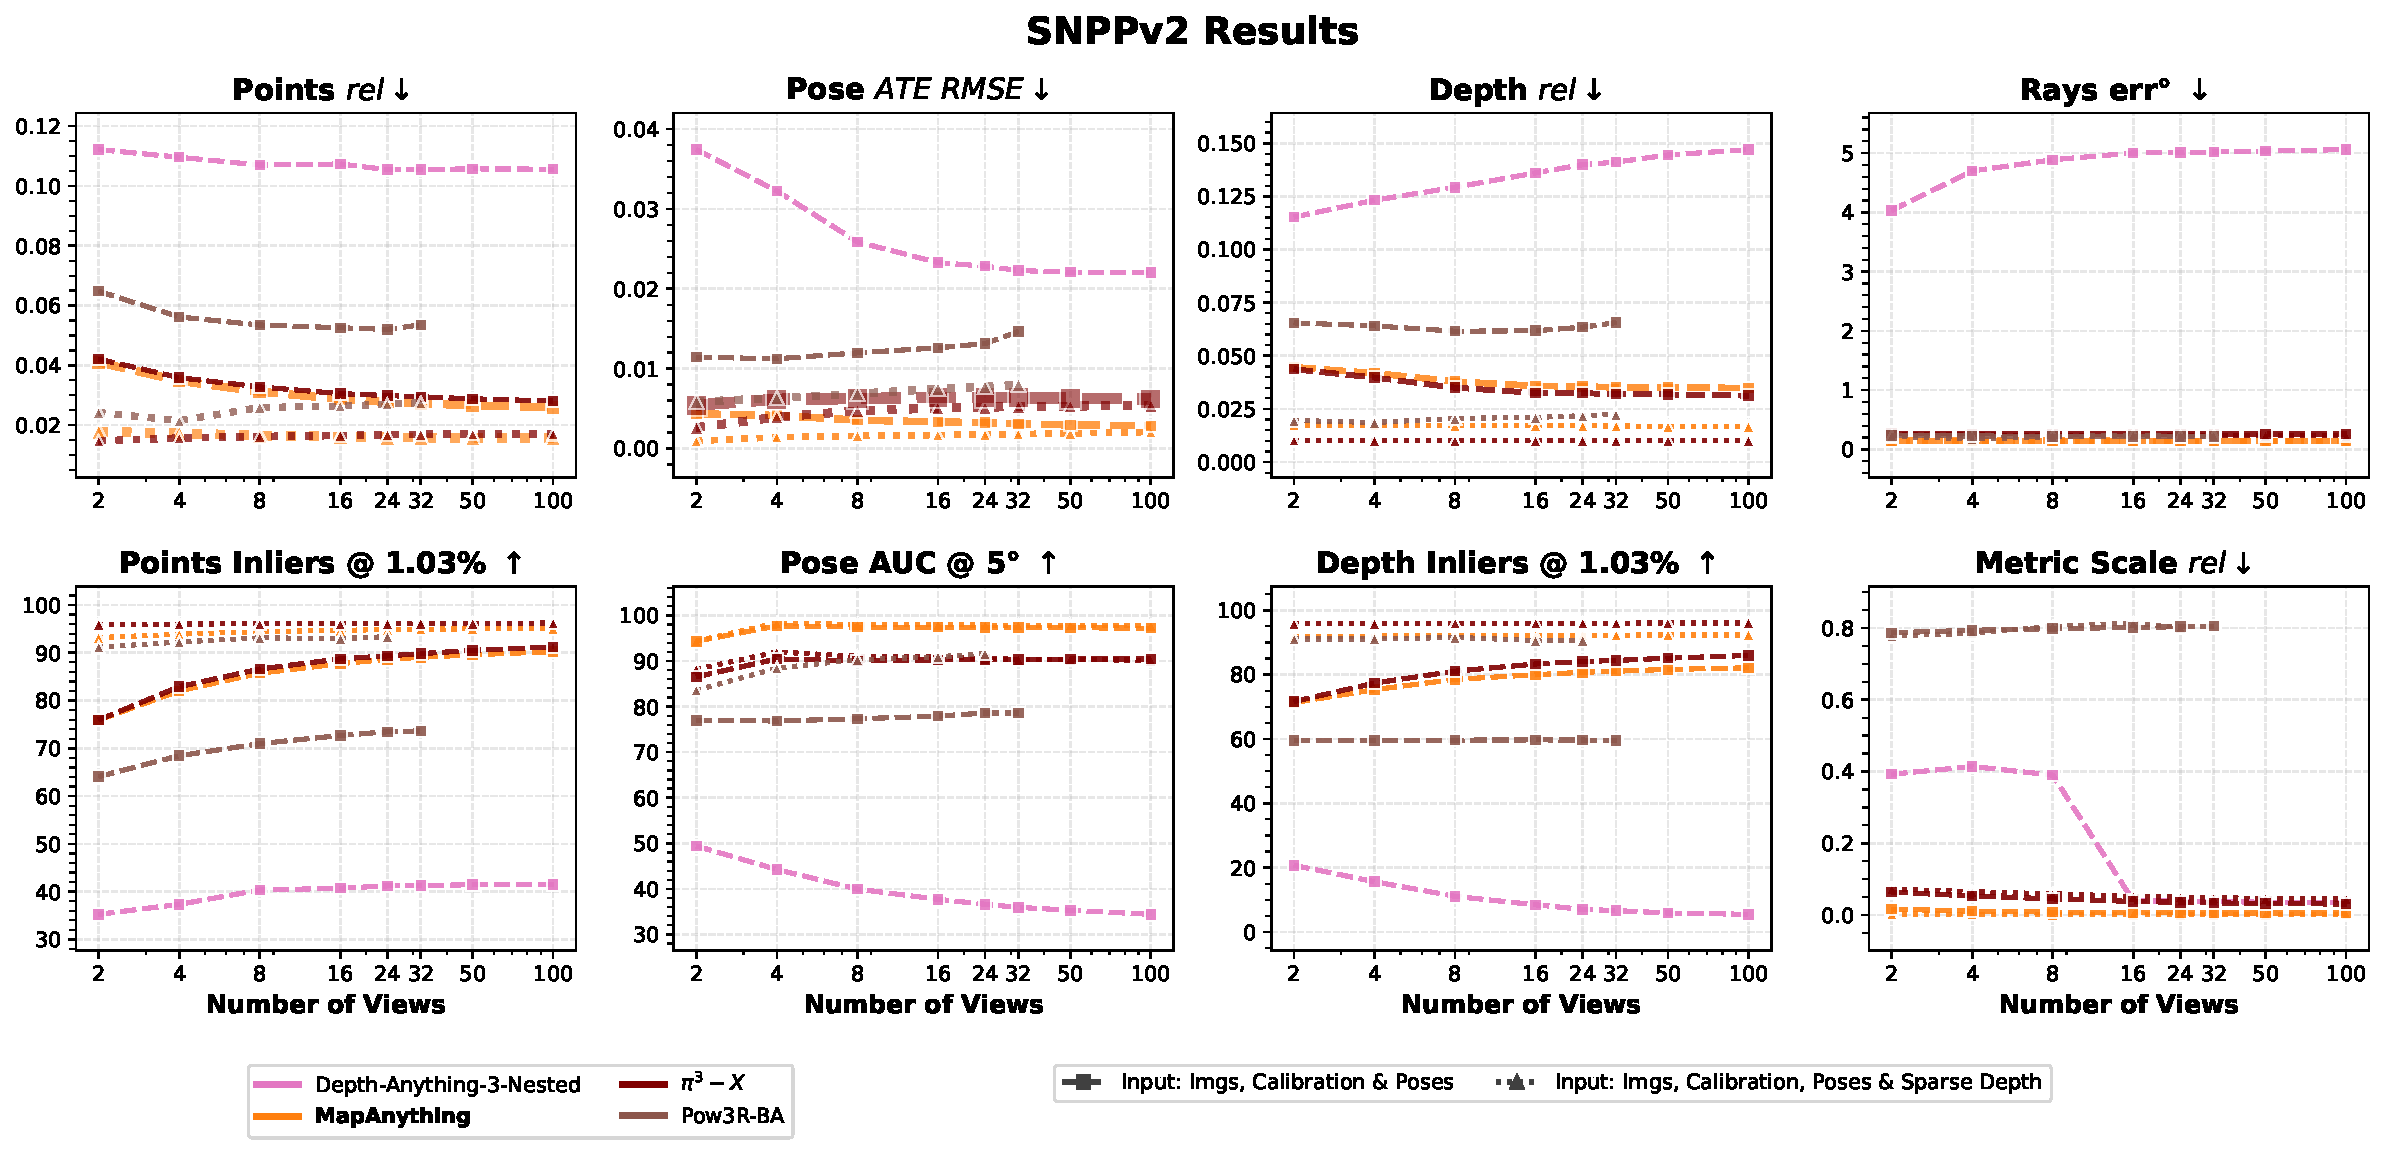
\includegraphics[trim={0cm 2cm 0cm 0cm},clip,width=0.9\linewidth]{figs/V1_1_Benchmarking/v1_1_bench_latest_multi_modal/results_v1_1_bench_latest_multi_modal_snppv2.pdf}

    \vspace{0.3em}
    
    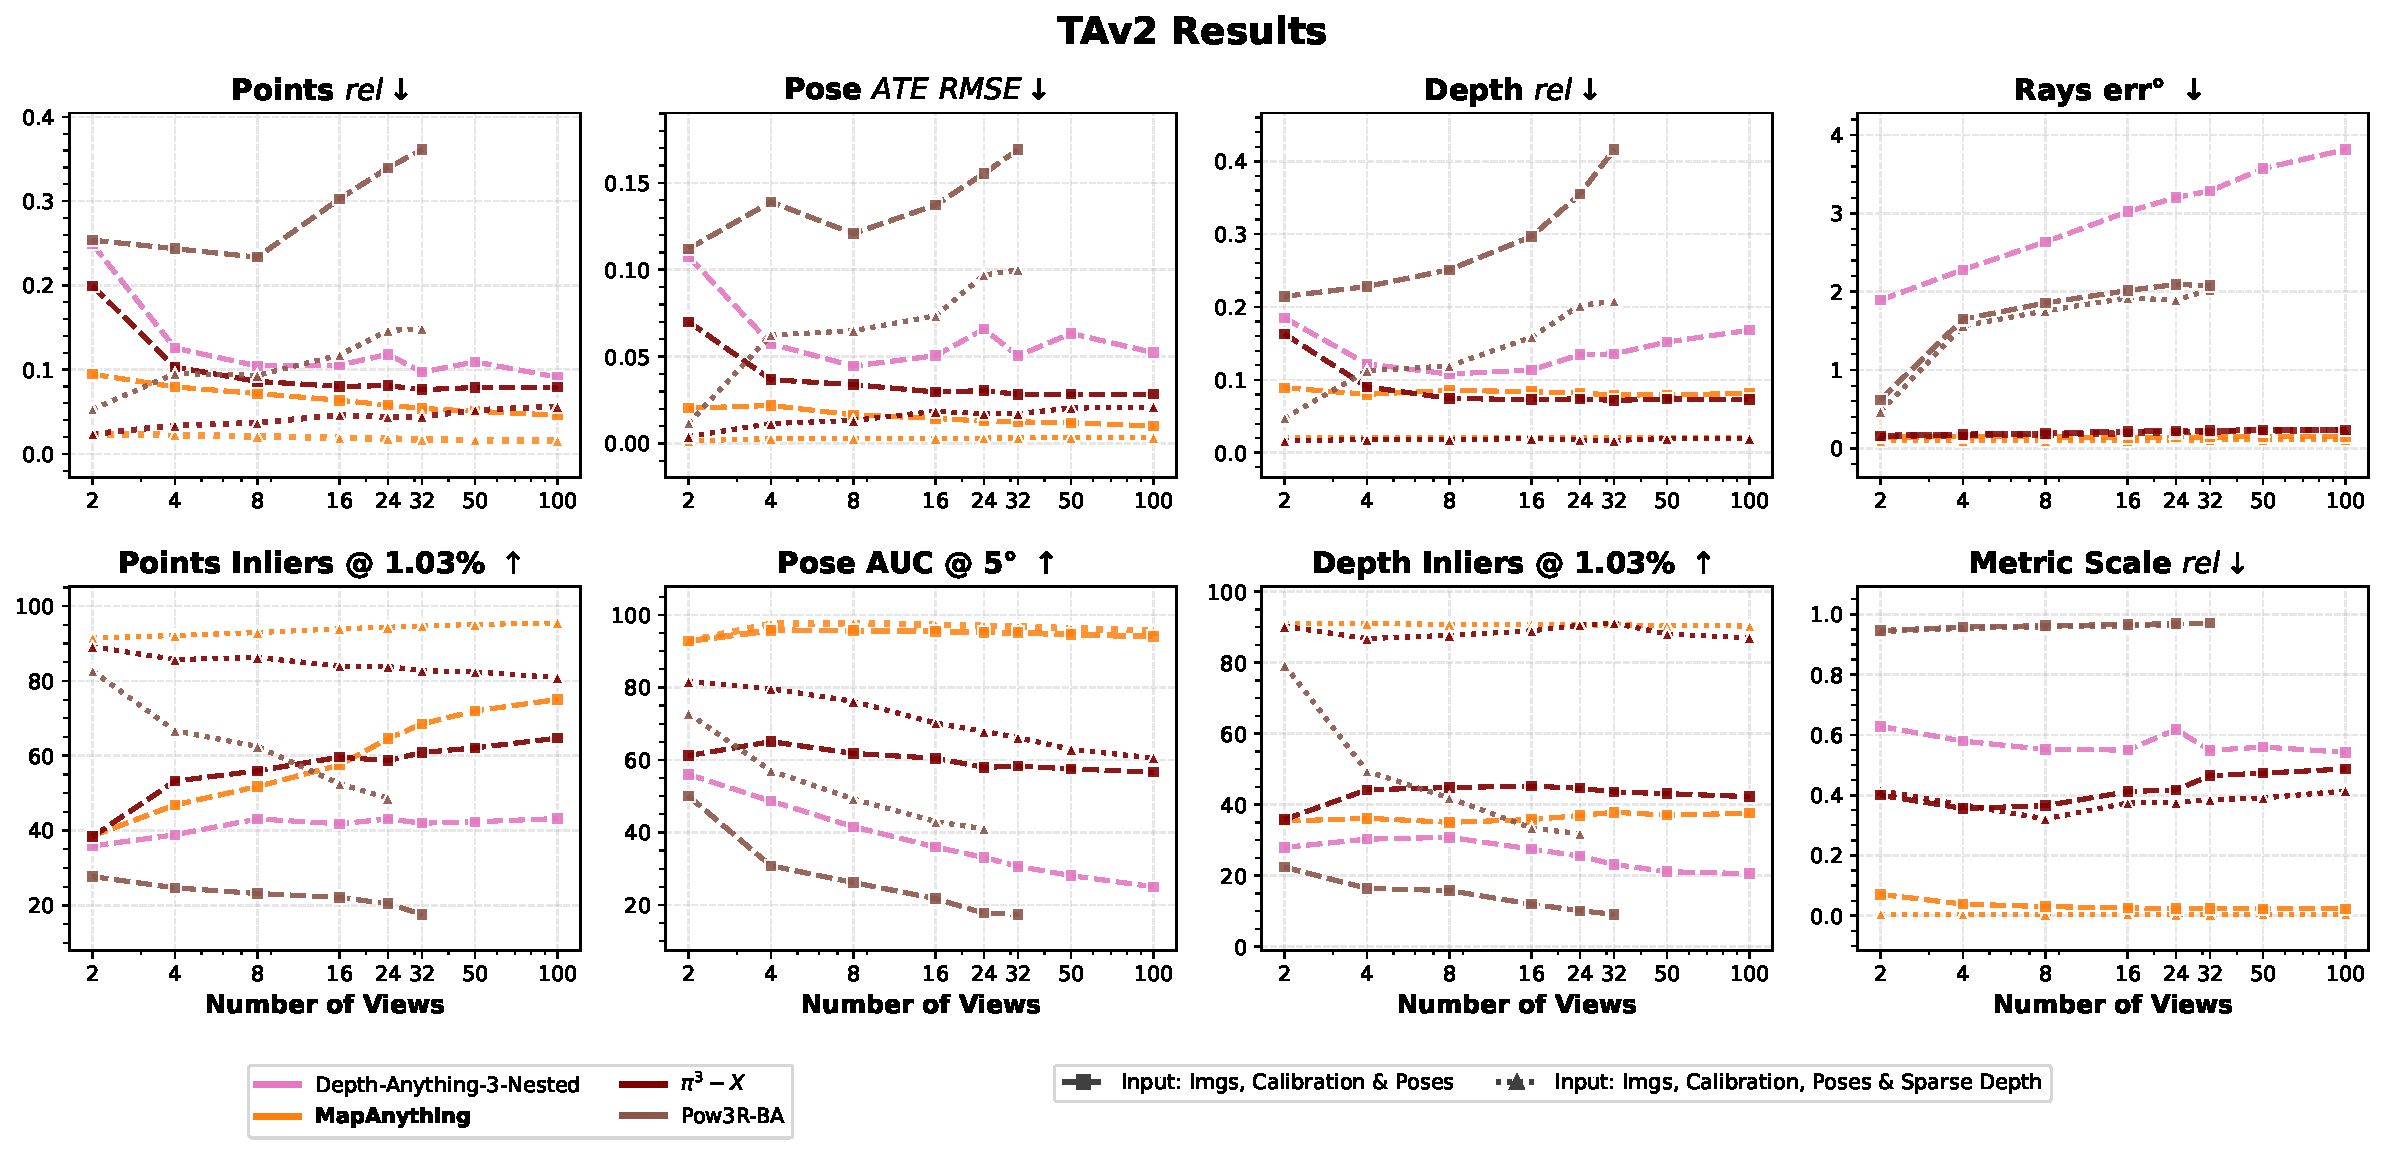
\includegraphics[trim={0cm 0cm 0cm 0cm},clip,width=0.9\linewidth]{figs/V1_1_Benchmarking/v1_1_bench_latest_multi_modal/results_v1_1_bench_latest_multi_modal_tav2.pdf}
    
    \caption{\label{fig:v1_1_bench_multi_modal_per_dataset}%
    \textbf{Dense multi-view reconstruction benchmarking across individual datasets using multi-modal inputs.}
    We also include results for latest public concurrent state-of-the-art models as of January 20th 2026.
    Please see \cref{fig:v1_1_bench_average} for details \& the averaged version.
    }
\end{figure*}



\clearpage
